\section{Conceituação}

\begin{frame}{Introdução}
	\begin{block}{O que é informática?}
		\begin{itemize}
			\item É o \textbf{tratamento automático da informação}, por meio da utilização de \textbf{técnicas}, \textbf{procedimentos} e \textbf{equipamentos adequados}, tendo por base os \textbf{computadores}.
			\item É a ciência do \textbf{tratamento racional} (especialmente por
			      máquinas automáticas) \textbf{da informação}, considerada como
			      \textbf{suporte dos conhecimentos humanos} e das \textbf{comunicações} nos
			      domínios \textbf{técnicos}, \textbf{econômicos} e \textbf{sociais}.
		\end{itemize}
	\end{block}

	\centering
	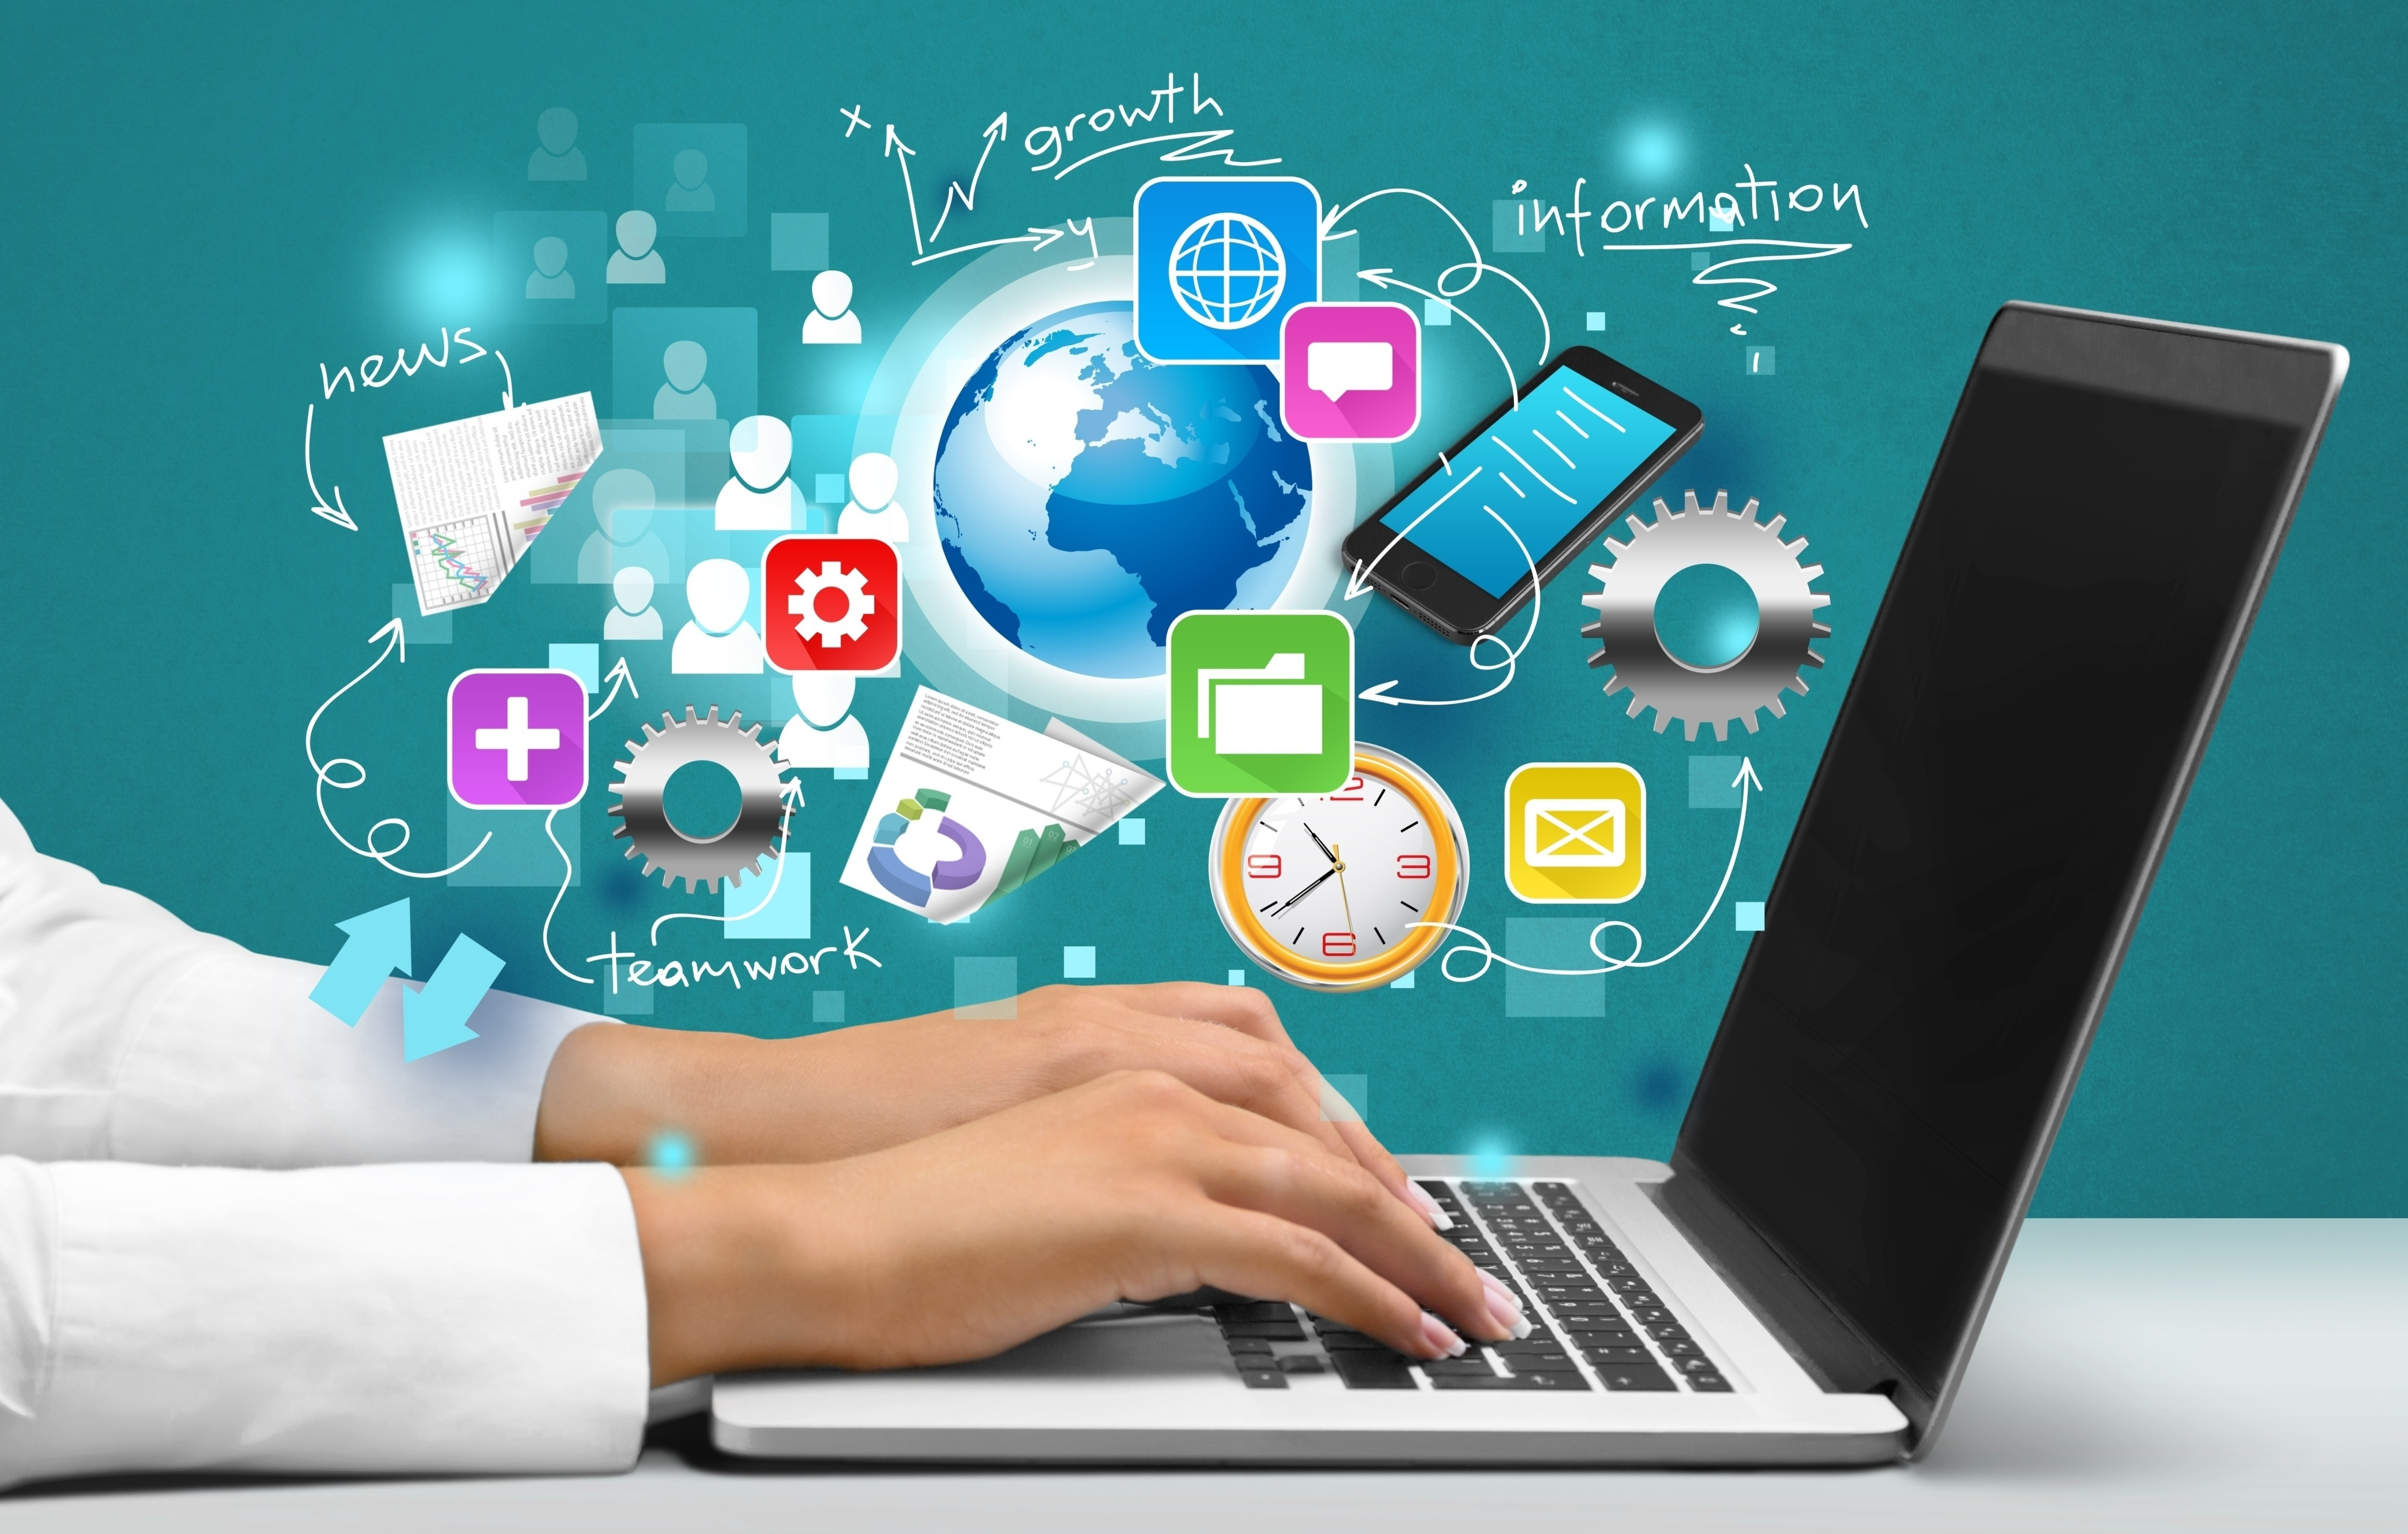
\includegraphics[width=0.45\linewidth]{Figuras/Ch01/fig1}

\end{frame}


\begin{frame}{Introdução}
	\centering
	\scalebox{1.2}{\begin{tikzpicture}[scale=0.5]
			\draw (-4,-3) rectangle (4,3); %CLP
		\draw (-4,0) -- (-2.5,0); %Div in out
		\draw (-2.5,-3) -- (-2.5,3); %Div cartoes
		\draw (-1.5,-2.5) rectangle (0,2.5); %Mem dados
		\draw (0.5,-2.5) rectangle (3.5,-1); %Mem prog
		\draw (1,0) rectangle (3,2); %CPU
		\draw (-4,-5) rectangle (4,-3); %Alimentacao
		\draw (-2.5,4) rectangle (4,6); %Term de prog
		
		\draw (1,2.6) node {CLP};
		
		\draw (-3.25,1.5) node[text width=1.5cm,align=center,rotate=90] {\small Cartões de input};
		
		\draw (-3.25,-1.5) node[text width=1.5cm,align=center,rotate=90] {\small Cartões de output};
		
		\node at (2,1) {\small CPU};
		
		\node[rotate=90,text width=1.5cm,align=center] at (-0.75,0) {\small Memória de dados};
		
		\node[text width=2cm,align=center] at (2,-1.75) {\footnotesize Memória de programa};
		
		\node at (-6,0) {Campo};
		
		\node at (0,-4) {Alimentação};
		
		\node[text width=3cm,align=center] at (0.75,5) {Terminal de programação};
		
		\draw[-Latex] (-8,1.5) -- node[above] {Entradas} +(4,0);
		\draw[Latex-] (-8,-1.5) -- node[below] {Saídas} +(4,0);
		\draw[-Latex] (-2.5,1.5) -- +(1,0);
		\draw[Latex-] (-2.5,-1.5) -- +(1,0);
		\draw[-Latex] (0,1.5) -- +(1,0);
		\draw[Latex-] (0,0.5) -- +(1,0);
		\draw[Latex-] (2,0) -- +(0,-1);
		
		\draw[-Latex] (-1.5,4) -- +(0,-1);
		\draw[Latex-] (3,4) -- +(0,-1);
	\end{tikzpicture}}
\end{frame}


\begin{frame}{O que são dados?}
	\begin{block}{}
		\begin{itemize}
			\item Dados são aquilo que pode ser manipulado, e que não necessariamente apresenta qualquer lógica.
			\item Informação é o produto que obtemos ao analisar e os dados, e é algo útil.
		\end{itemize}
	\end{block}

	\bigskip

	\centering
	
\includegraphics[width=1\linewidth]{Figuras/Ch01/fig1.1}
\end{frame}


\begin{frame}{O que é um computador?}
	\begin{block}{}
		\begin{itemize}
			\item É o elemento físico utilizado para o tratamento de dados e obtenção da informação.
			\item É uma máquina constituída por uma série de componentes e circuitos eletrônicos, capaz de receber, armazenar, processar e transmitir informações.
			\item É uma \textbf{máquina programável}, capaz de realizar uma
			      grande variedade de tarefas seguindo uma sequência de
			      comandos de acordo com o que for especificado.
		\end{itemize}
	\end{block}

	\centering
	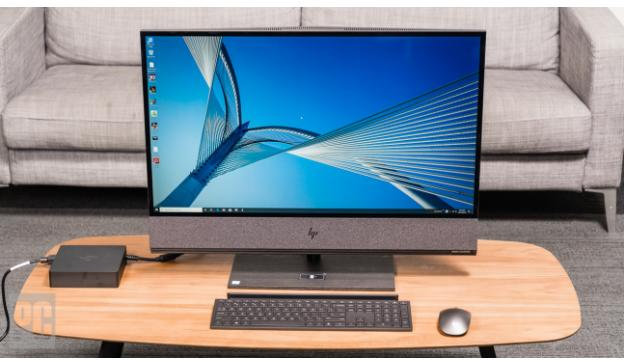
\includegraphics[width=0.45\linewidth]{Figuras/Ch01/fig2}
\end{frame}


\begin{frame}{Características fundamentais do computador}
	\begin{block}{Automático}
		\begin{itemize}
			\item Manipula os dados sem necessidade de intervenção humana.
		\end{itemize}
	\end{block}

	\medskip

	\centering
	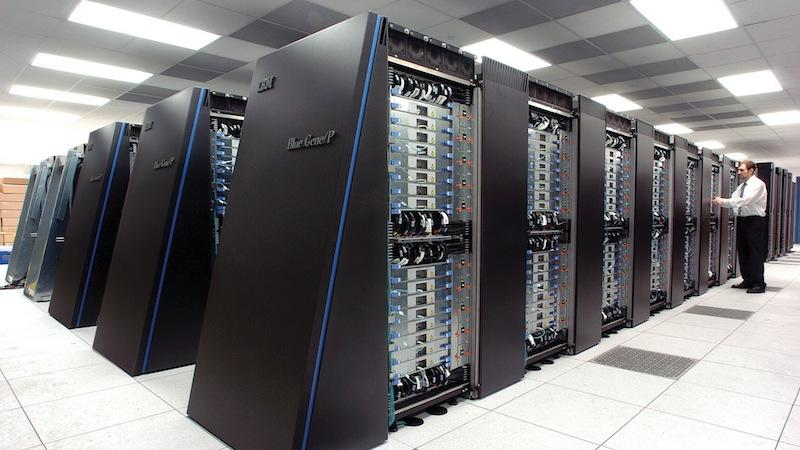
\includegraphics[width=0.8\linewidth]{Figuras/Ch01/fig3}
\end{frame}


\begin{frame}{Características fundamentais do computador}
	\begin{block}{Universal}
		\begin{itemize}
			\item Executa qualquer tarefa desde que descrita por um programa.
		\end{itemize}
	\end{block}

	\centering
	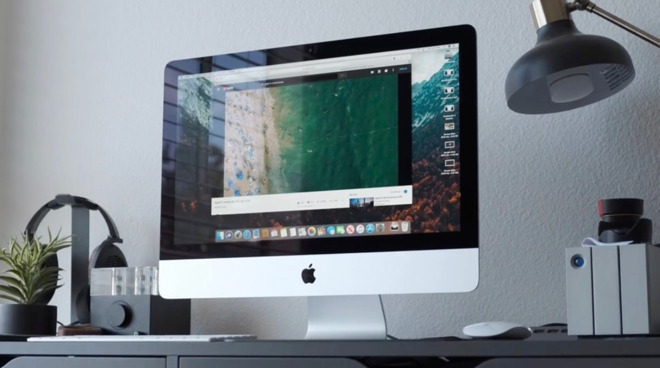
\includegraphics[width=0.6\linewidth]{Figuras/Ch01/fig4.1}
\end{frame}


\begin{frame}{Características fundamentais do computador}
	\begin{block}{Eletrônico}
		\begin{itemize}
			\item Usa componentes eletrônicos para manipular e representar os dados.
		\end{itemize}
	\end{block}

	\centering
	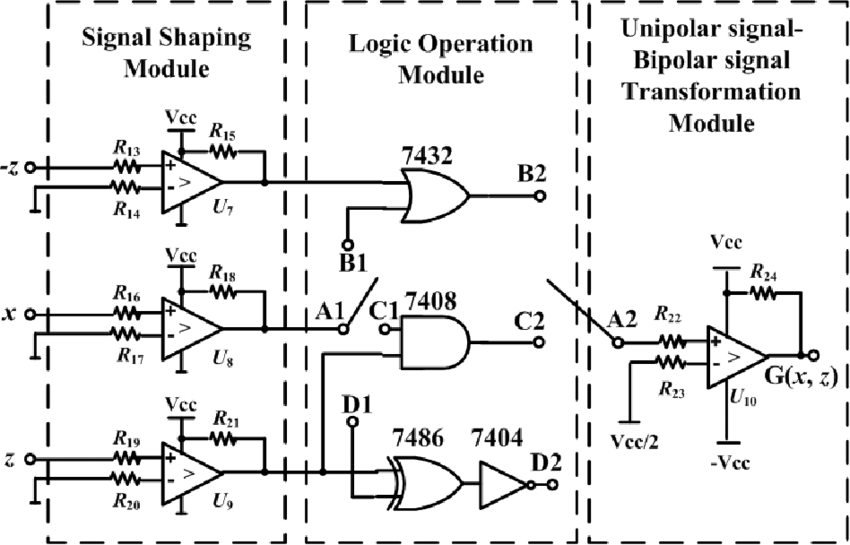
\includegraphics[width=0.7\linewidth]{Figuras/Ch01/fig6}
\end{frame}


\begin{frame}{Características fundamentais do computador}
	\centering
	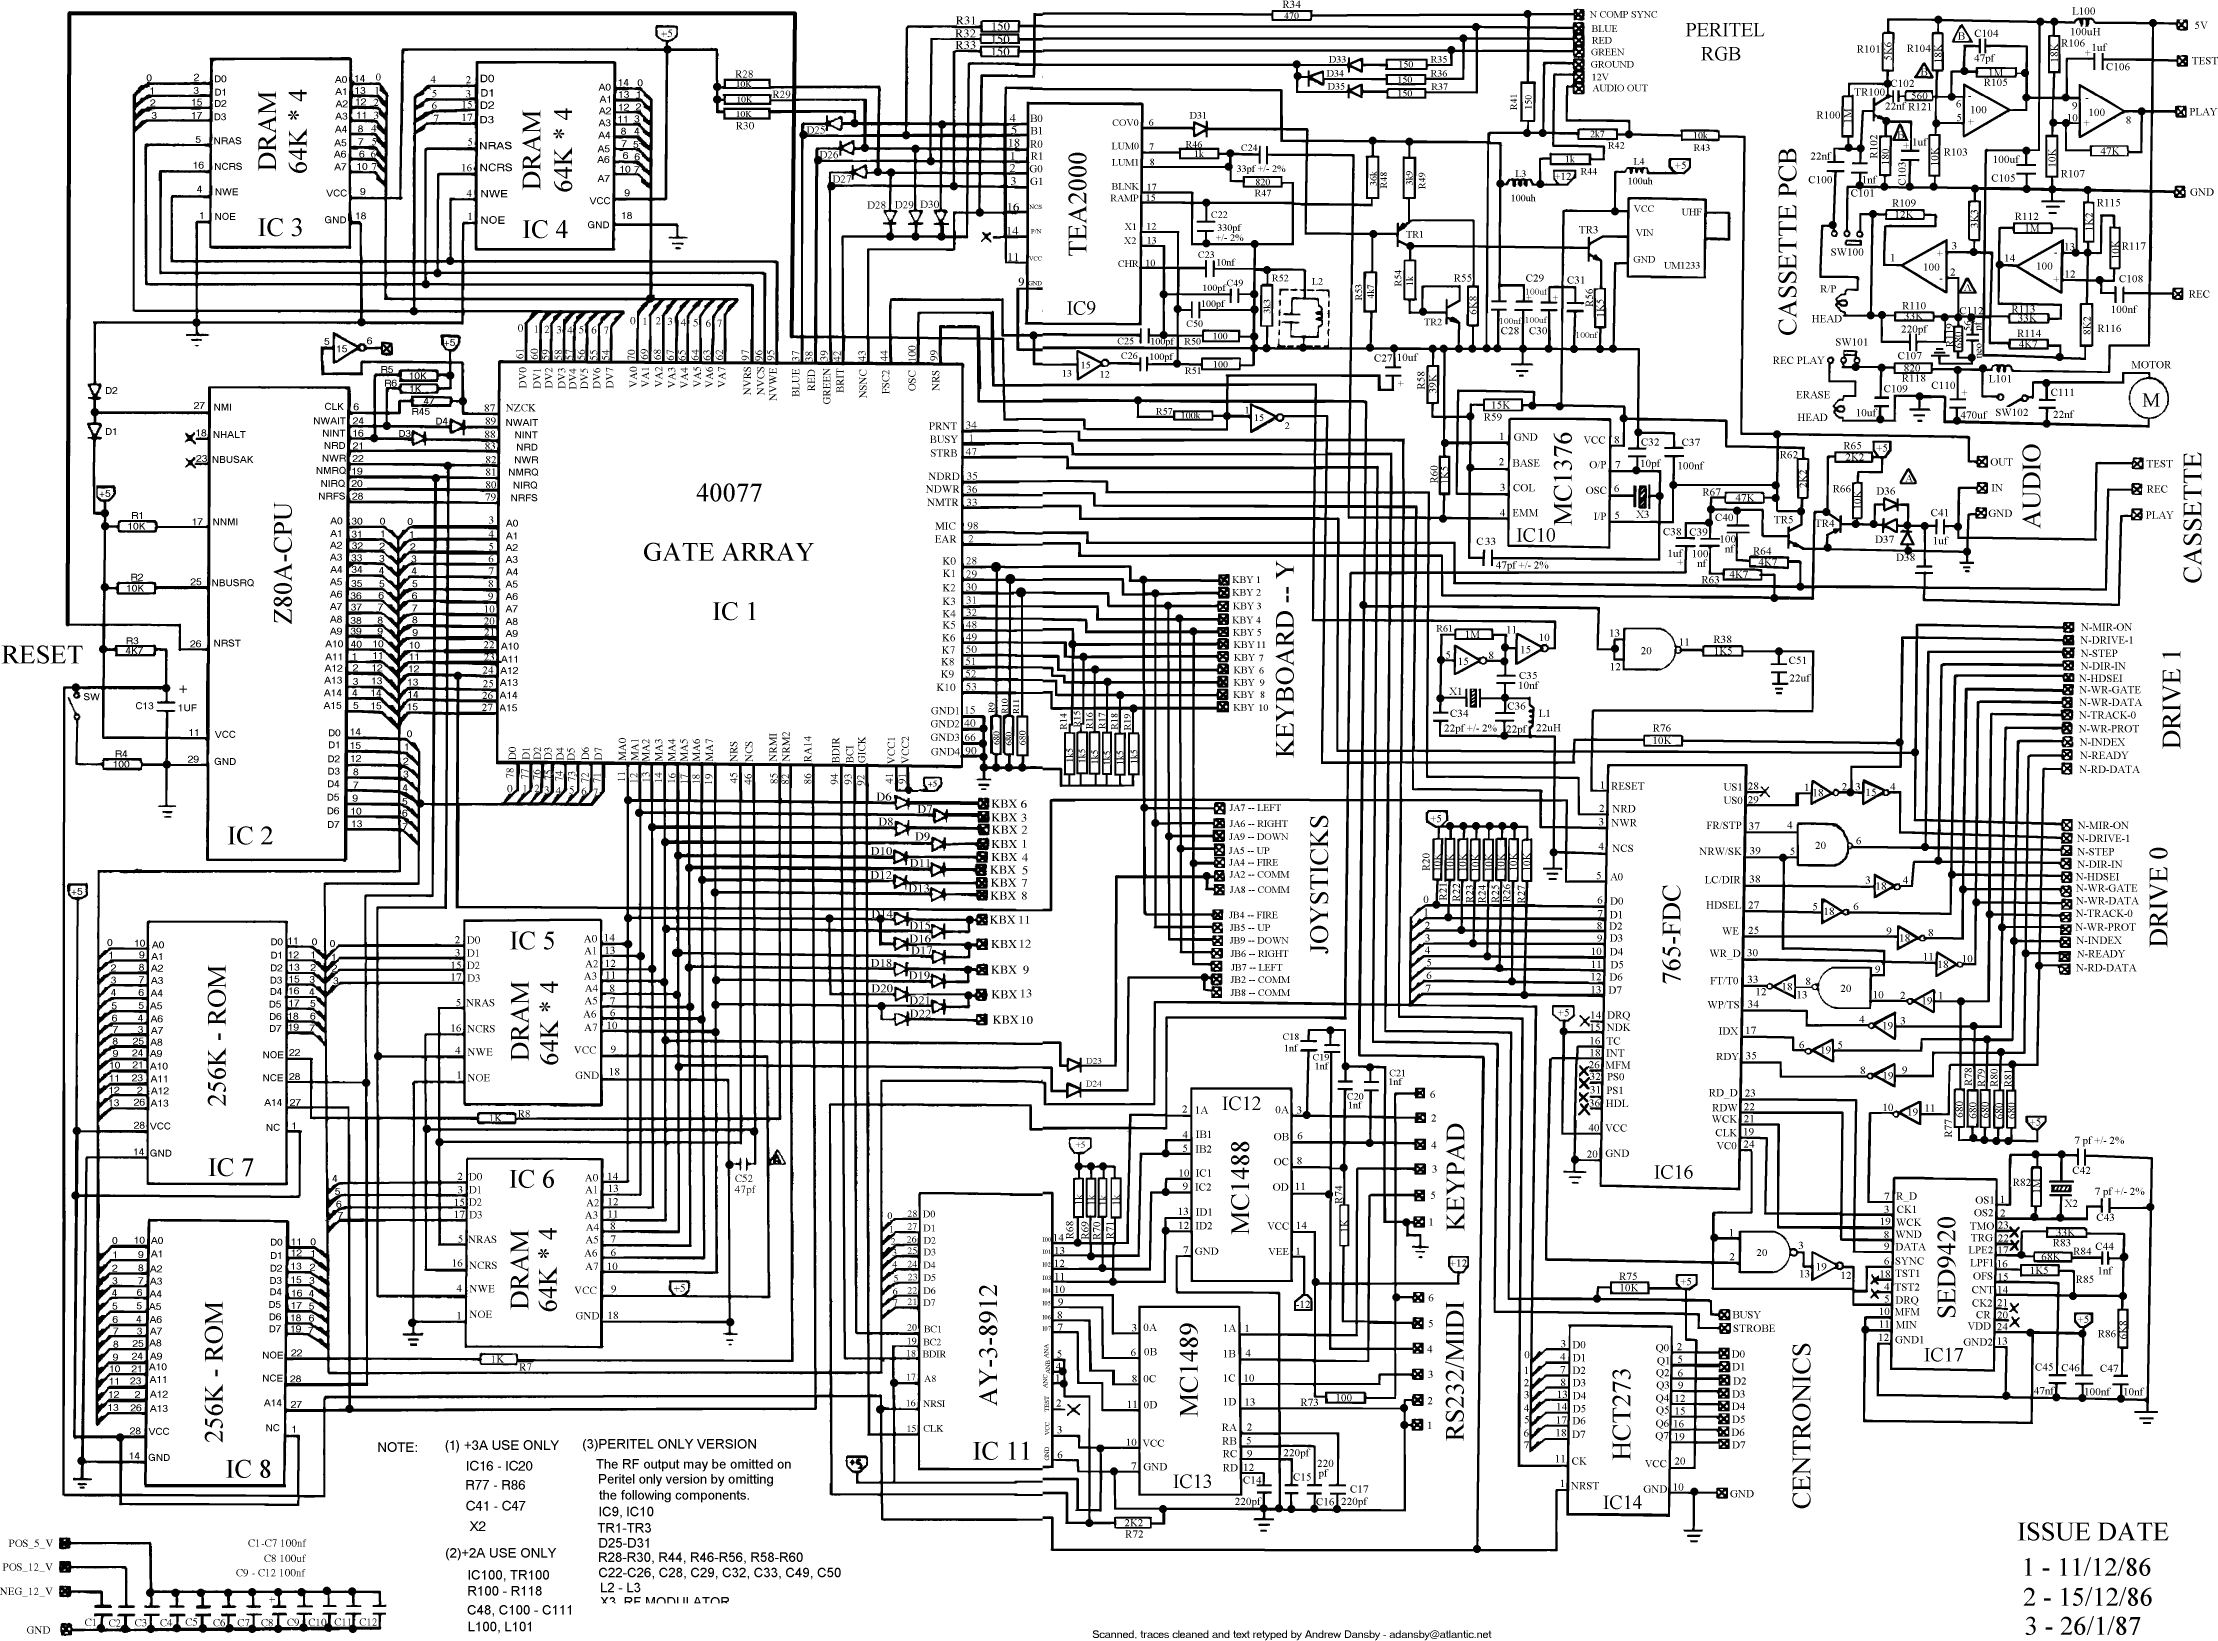
\includegraphics[width=0.85\linewidth]{Figuras/Ch01/fig7}
\end{frame}


\begin{frame}{Características fundamentais do computador}
	\begin{block}{Digital}
		\begin{itemize}
			\item Representa os dados como dígitos binários.
		\end{itemize}
	\end{block}

	\vspace{1cm}

	\centering
	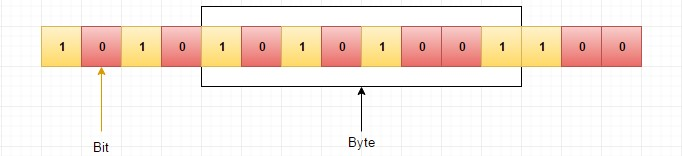
\includegraphics[width=1\linewidth]{Figuras/Ch01/fig9}
\end{frame}


\begin{frame}{Características fundamentais do computador}
	\centering
	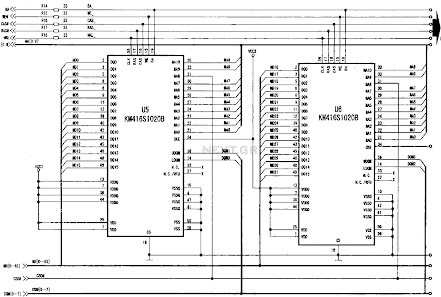
\includegraphics[width=0.8\linewidth]{Figuras/Ch01/fig8}
\end{frame}


\begin{frame}{Vantagens do uso de um computador}
	\begin{block}{}
		\begin{itemize}
			\item \textbf{Velocidade:} Executa operações em pequenas frações de tempo.
			\item \textbf{Aumento de  Produtividade:} Economia de tempo.
			\item \textbf{Confiabilidade:} Executa as tarefas exatamente como lhe são ordenadas.
			\item \textbf{Versatilidade:} Possibilidade de realizar uma infinidade de trabalhos de diferentes tipos.
		\end{itemize}
	\end{block}
\end{frame}


\begin{frame}{Vantagens do uso de um computador}
	\begin{block}{Outras vantagens}
		\begin{itemize}
			\item Capacidade de armazenamento.
			\item Melhoria na qualidade da informação produzida.
			\item Eficiência no armazenamento e consulta da informação.
			\item Liberação das pessoas de tarefas rotineiras.
		\end{itemize}
	\end{block}
\end{frame}


\begin{frame}{Tipos de computadores}
	\begin{block}{Máquinas com lógica predeterminada}
		O algoritmo é intrínseco aos seus circuitos (calculadora, bomba de gasolina, relógio, etc.).
	\end{block}

	\centering
	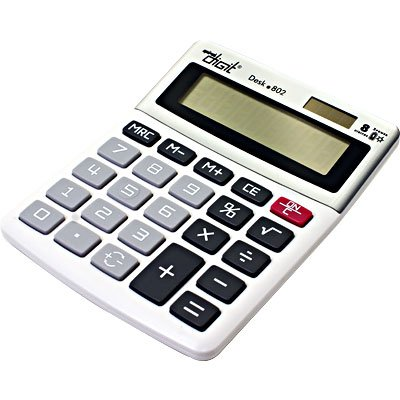
\includegraphics[width=0.5\linewidth]{Figuras/Ch01/fig10}
\end{frame}


\begin{frame}{Tipos de computadores}
	\begin{block}{Máquinas com lógica programada}
		Admitem programação (computadores convencionais).
	\end{block}

	\medskip

	\centering
	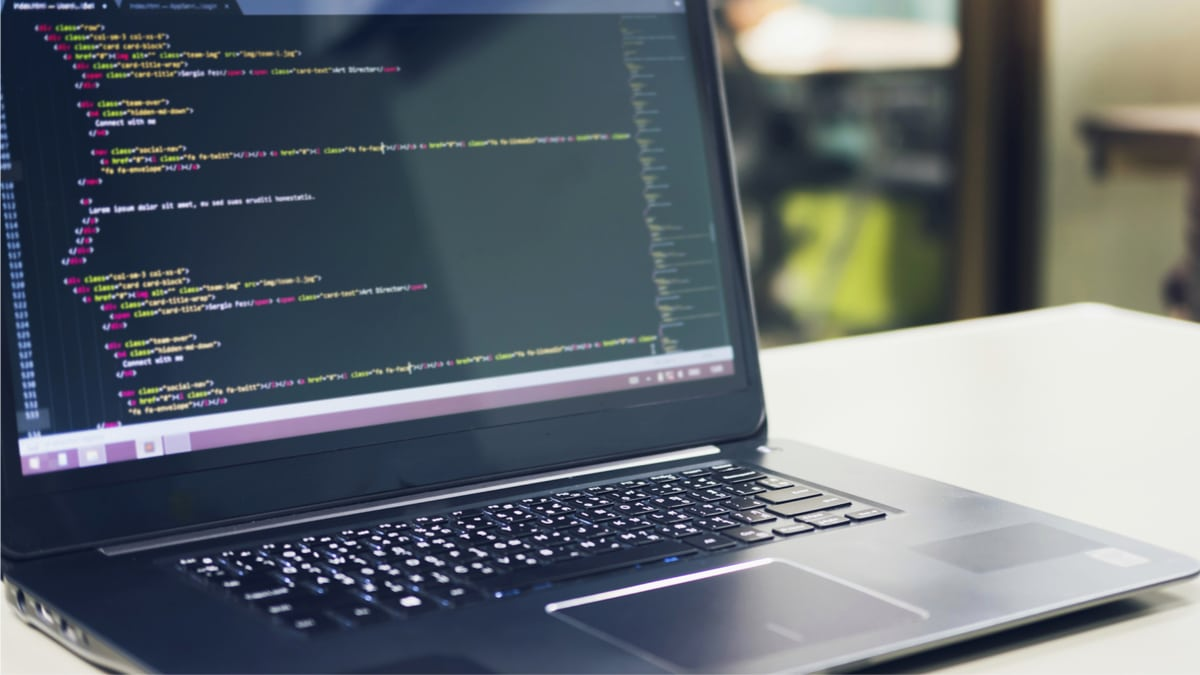
\includegraphics[width=0.9\linewidth]{Figuras/Ch01/fig11}
\end{frame}


\begin{frame}{Classificação quanto à utilização}
	\begin{block}{}
		\begin{itemize}
			\item \textbf{Científicos:} Pesquisas científicas de altíssima precisão.
			\item \textbf{Comerciais:} Aplicações comerciais; Alto volume de entrada e saída de dados.
			\item \textbf{Pessoais:} Uso de tarefas pessoais, comunicação, trabalho e entretenimento.
		\end{itemize}
	\end{block}

	\bigskip

	\begin{minipage}{0.49\linewidth}
		\centering
		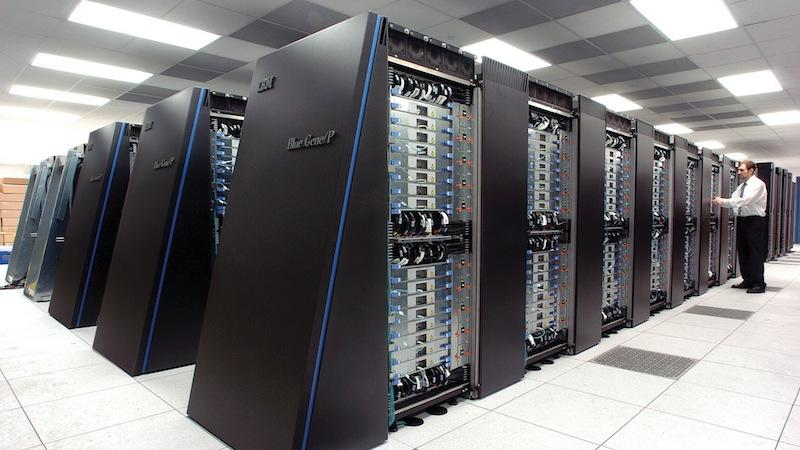
\includegraphics[width=1\linewidth]{Figuras/Ch01/fig3}
	\end{minipage}\hfill
	\begin{minipage}{0.49\linewidth}
		\centering
		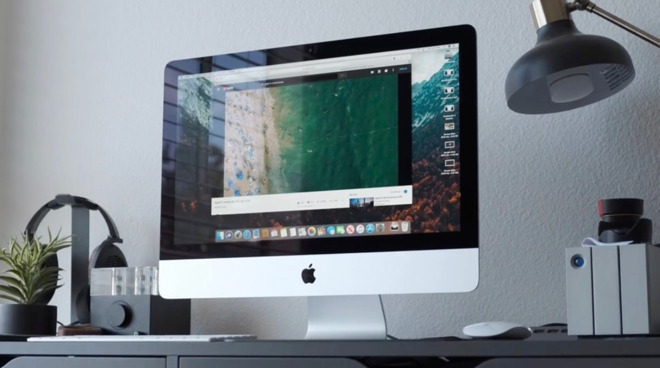
\includegraphics[width=0.9\linewidth]{Figuras/Ch01/fig4.1}
	\end{minipage}

\end{frame}


\begin{frame}{Aplicações de computadores}
	\begin{block}{Entretenimento}
		\begin{itemize}
			\item Redes sociais, música, cinema, jogos, etc.
		\end{itemize}
	\end{block}

	\bigskip

	\centering
	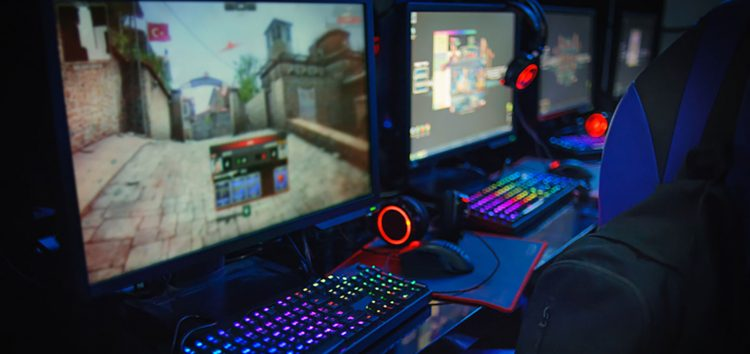
\includegraphics[width=1\linewidth]{Figuras/Ch01/fig12}
\end{frame}


\begin{frame}{Aplicações de computadores}
	\begin{block}{No lar}
		\begin{itemize}
			\item Eletrodométicos informatizados, segurança, etc.
		\end{itemize}
	\end{block}

	\bigskip

	\centering
	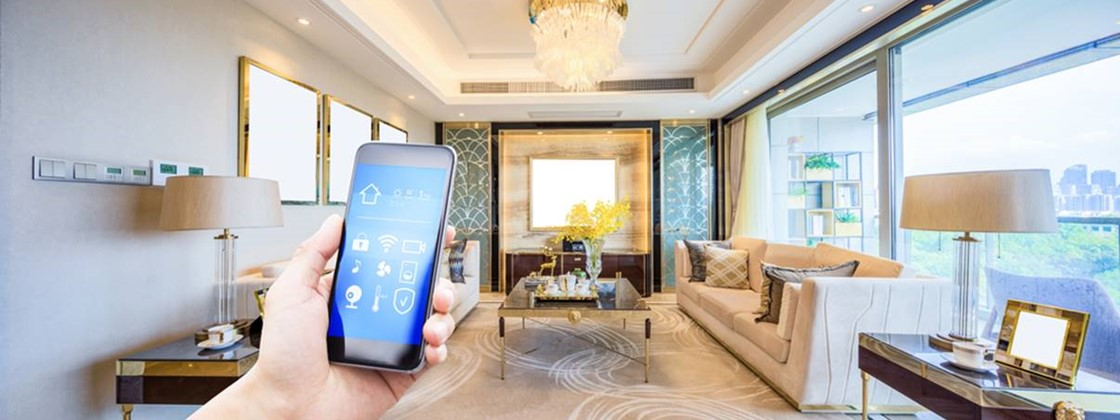
\includegraphics[width=1\linewidth]{Figuras/Ch01/fig13}
\end{frame}


\begin{frame}{Aplicações de computadores}
	\begin{block}{Comercial}
		\begin{itemize}
			\item Sistemas de pagamentos, controle de estoque, cobranças, etc.
		\end{itemize}
	\end{block}

	\bigskip

	\centering
	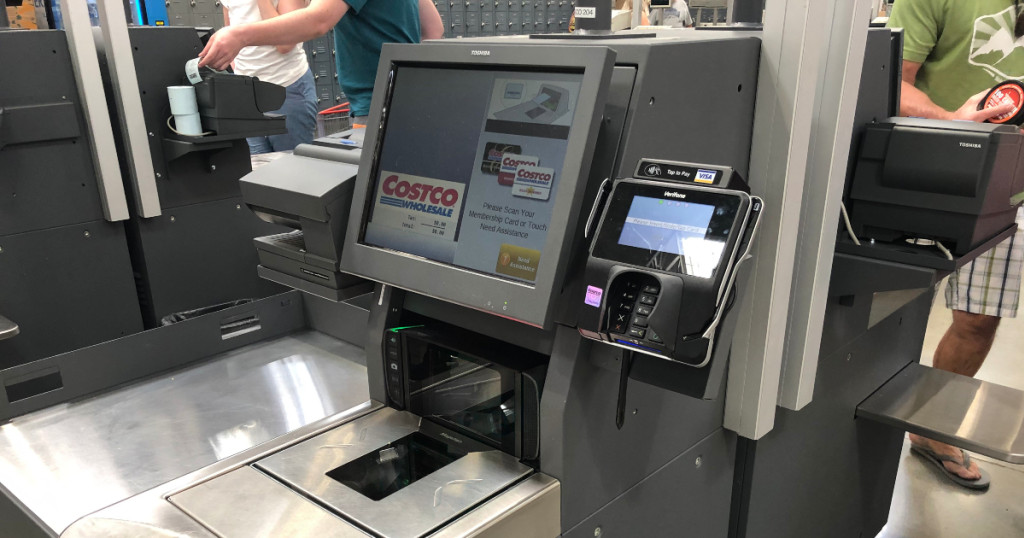
\includegraphics[width=0.9\linewidth]{Figuras/Ch01/fig15}
\end{frame}


\begin{frame}{Aplicações de computadores}
	\begin{block}{Instrumentação}
		\begin{itemize}
			\item Equipamentos de laboratório, microscópios, etc.
		\end{itemize}
	\end{block}

	\centering
	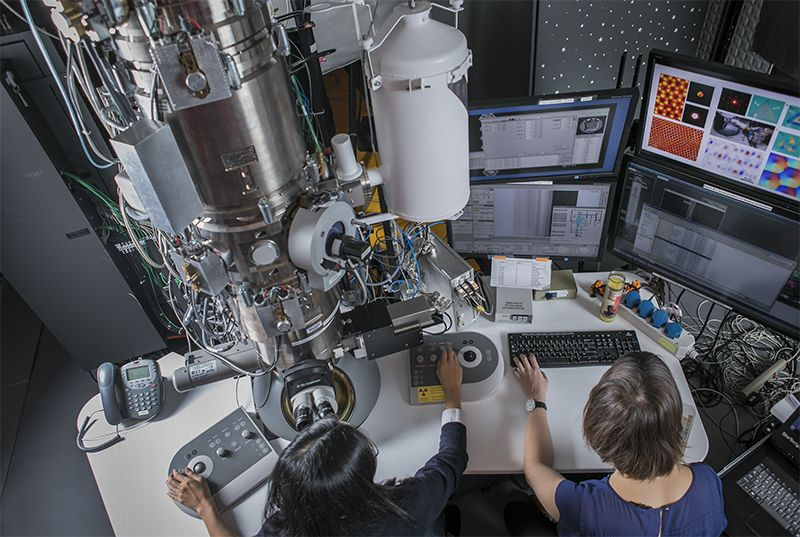
\includegraphics[width=0.7\linewidth]{Figuras/Ch01/fig14}
\end{frame}


\begin{frame}{Aplicações de computadores}
	\begin{block}{Controle de processos}
		\begin{itemize}
			\item Centrais telefônicas, controle de tráfego aéreo, controle de segurança de cidades, controle de refinarias, etc.
		\end{itemize}
	\end{block}

	\centering
	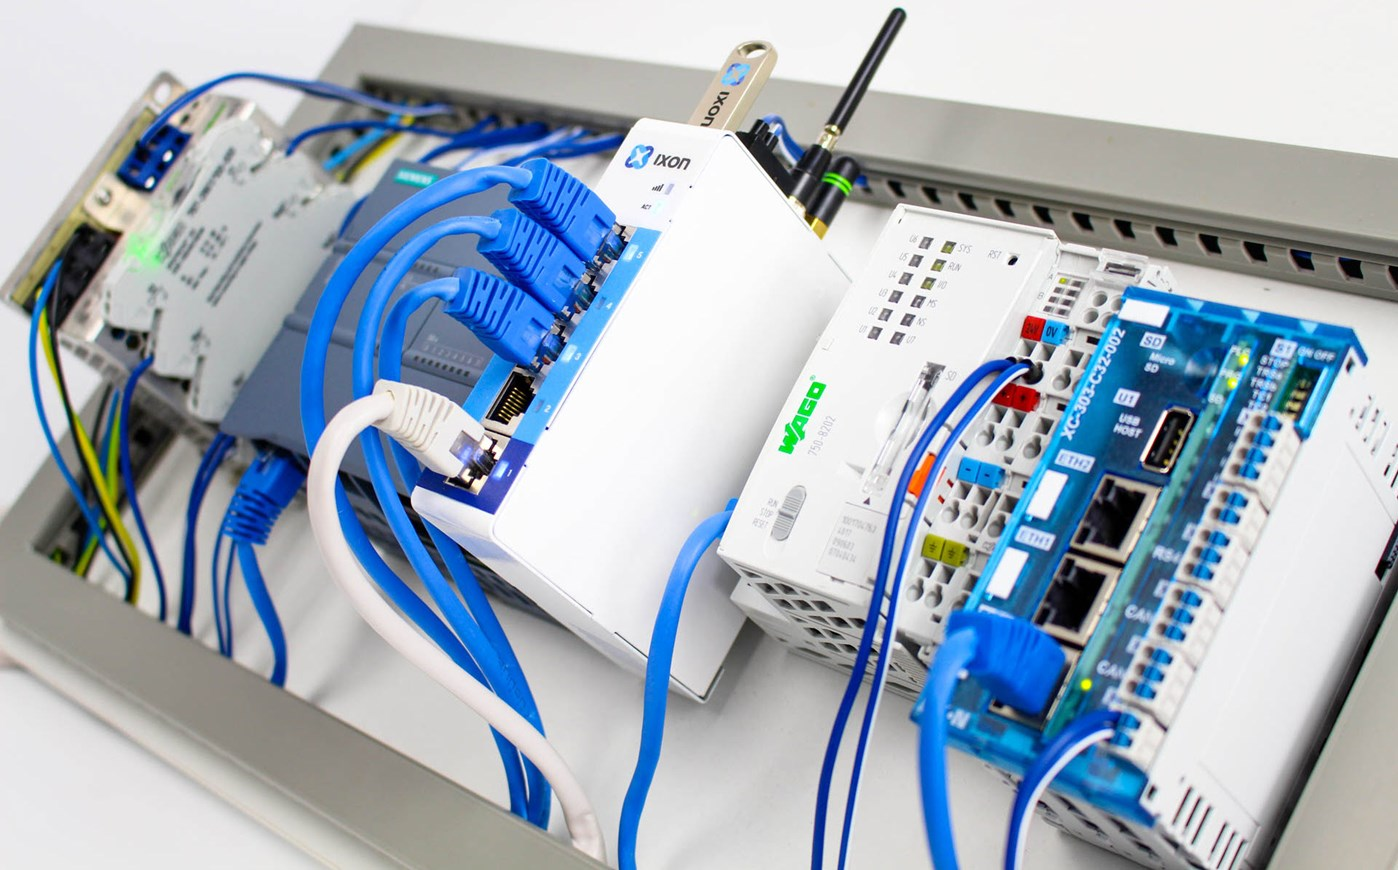
\includegraphics[width=0.7\linewidth]{Figuras/Ch01/fig16}
\end{frame}


\begin{frame}{Aplicações de computadores}
	\begin{block}{Medicina}
		\begin{itemize}
			\item Diagnóstico de doenças, diagnósticos de imagens, monitoramento de pacientes, cirurgia auxiliada por computador, etc.
		\end{itemize}
	\end{block}

	\centering
	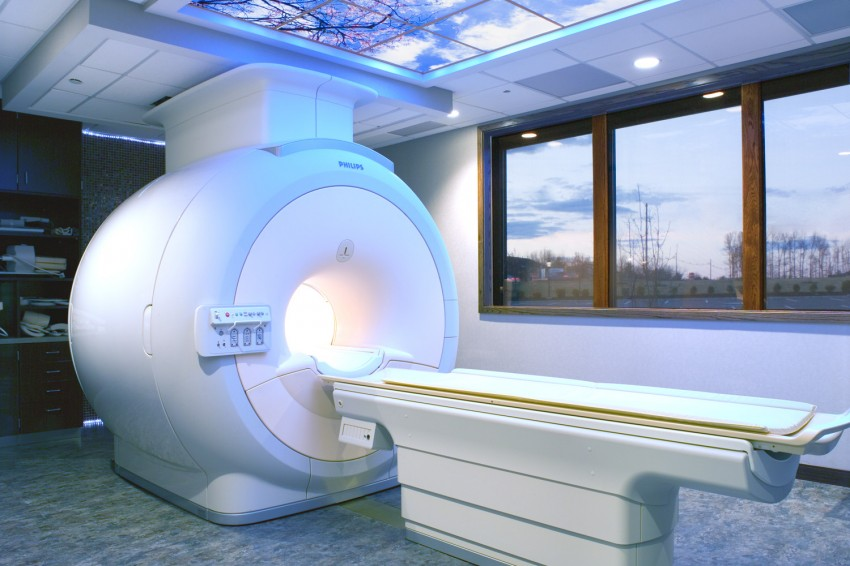
\includegraphics[width=0.7\linewidth]{Figuras/Ch01/fig17}
\end{frame}


\begin{frame}{Aplicações de computadores}
	\begin{block}{Educação}
		\begin{itemize}
			\item Ensino à distância, bibliotecas digitais, aulas, museus digitais, etc.
		\end{itemize}
	\end{block}

	\bigskip

	\centering
	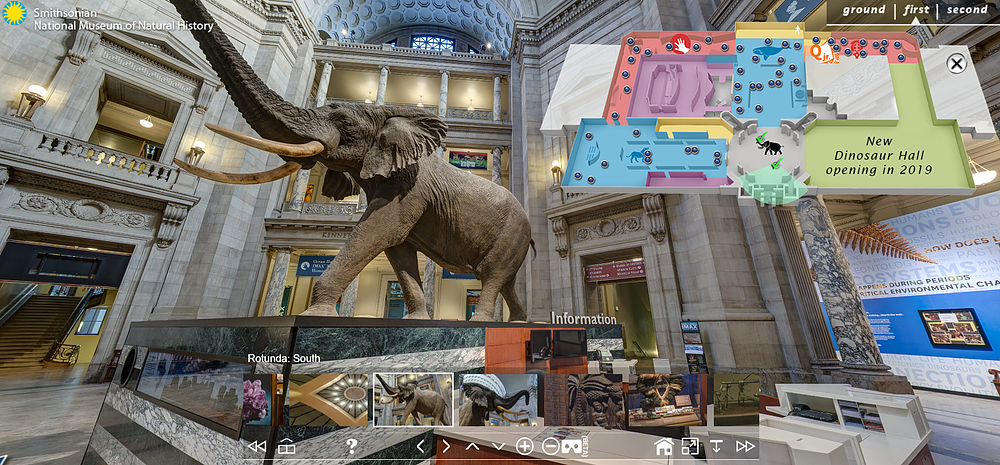
\includegraphics[width=1\linewidth]{Figuras/Ch01/fig18}
\end{frame}


\begin{frame}{Aplicações de computadores}
	\begin{block}{Engenharia e Arquitetura}
		\begin{itemize}
			\item CAD, projetos 3D, cálculos complexos, etc.
		\end{itemize}
	\end{block}

	\centering
	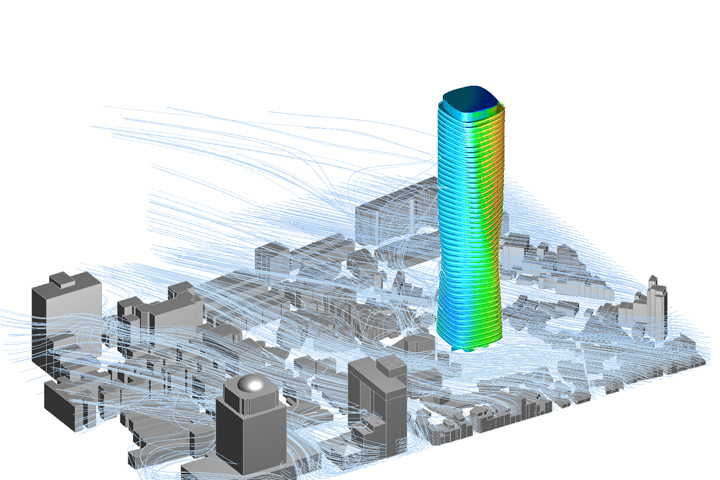
\includegraphics[width=0.75\linewidth]{Figuras/Ch01/fig19}
\end{frame}


\begin{frame}{O operador}
	\begin{block}{}
		\begin{itemize}
			\item Pessoa responsável pelo manuseio do computador.
			\item Deve possuir \textbf{habilidades} em:
			      \begin{itemize}
				      \item\normalsize Uso de sistemas operacionais, ferramentas de produtividade (softwares de escritório) e aplicativos específicos.
				      \item\normalsize Digitação e redação de documentos e relatórios.
				      \item\normalsize Manutenção.
			      \end{itemize}

		\end{itemize}
	\end{block}
\end{frame}


\begin{frame}{Classificação dos computadores}
	\begin{block}{Computador pessoal (\textit{PC})}
		\begin{itemize}
			\item É um computador que possui um baixo custo e que se destina ao uso individual ou de um pequeno grupo de pessoas.
		\end{itemize}
	\end{block}

	\centering
	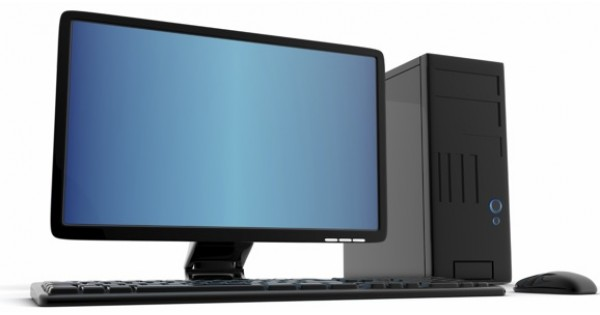
\includegraphics[width=0.8\linewidth]{Figuras/Ch01/fig2.1}
\end{frame}


\begin{frame}{Classificação dos computadores}
	\begin{block}{\textit{Notebook} (ou \textit{Laptop})}
		\begin{itemize}
			\item Com tamanho reduzido, tem as mesmas funcionalidades de um computador de mesa e iguala-se em tecnologia.
			\item Grande variedades de modelos.
			\item Muito úteis devido à sua \textbf{portabilidade}.
		\end{itemize}
	\end{block}

	\centering
	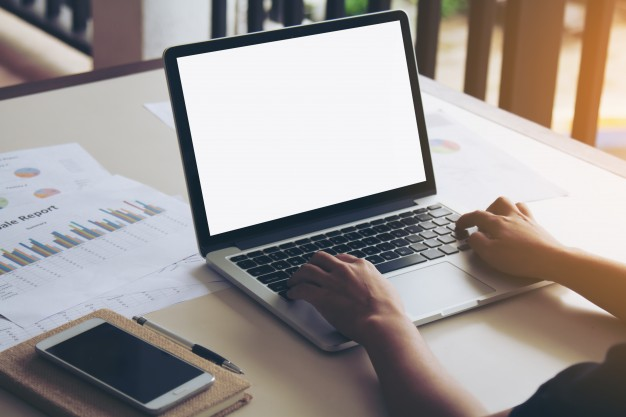
\includegraphics[width=0.6\linewidth]{Figuras/Ch01/fig3.1}
\end{frame}


\begin{frame}{Classificação de computadores}
	\begin{block}{\textit{Handheld}}
		\begin{itemize}
			\item Denominados Personal Digital Assistants (PDA's).
			\item Normalmente são utilizados em tarefas mais simples.
			\item Cada vez mais estão sendo \textbf{substituídos por \textit{smartphones }e \textit{tablets}}.
			\item Uteis para entregadores, garçons, etc.
		\end{itemize}
	\end{block}

	\medskip

	\centering
	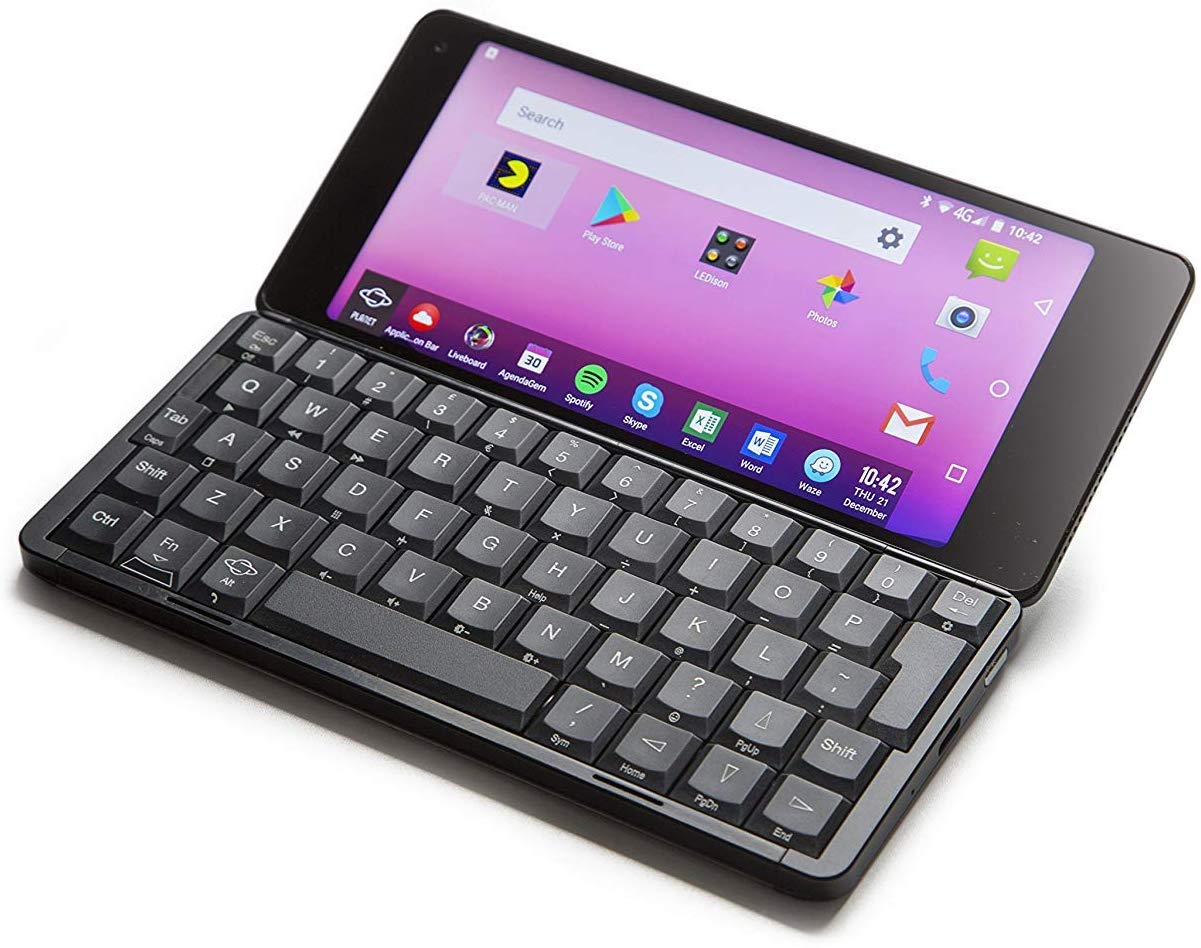
\includegraphics[width=0.45\linewidth]{Figuras/Ch01/fig21}
\end{frame}


\begin{frame}{Classificação de computadores}
	\begin{block}{\textit{Mainframe}}
		\begin{itemize}
			\item São grandes computadores, capazes de ocupar salas inteiras.
			\item Mais conhecidos como \textit{servidores corporativos}.
			\item São empregados em ambientes que devem processar \textbf{grande volume de
				      informações}.
		\end{itemize}
	\end{block}

	\centering
	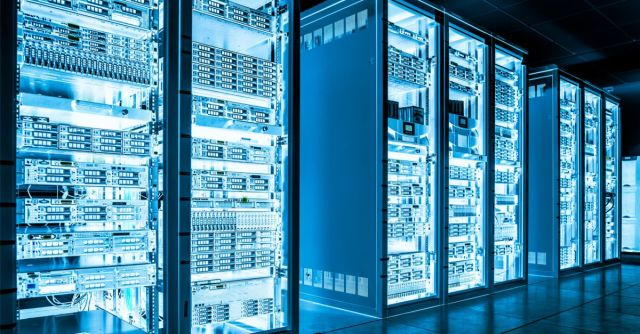
\includegraphics[width=0.7\linewidth]{Figuras/Ch01/fig5.1}
\end{frame}


\begin{frame}{Conceitos de hardware e software}
	\begin{block}{Sistema Operacional}
		\begin{itemize}
			\item O principal e mais importante software é o \textit{Sistema
				      Operacional} (SO), pois é ele quem “dá vida” ao hardware e
			      fornece as bases para a execução de programas.
			\item Windows, Linux, MacOS, Android, iOS são exemplos de
			      SO's.
		\end{itemize}
	\end{block}

	\centering
	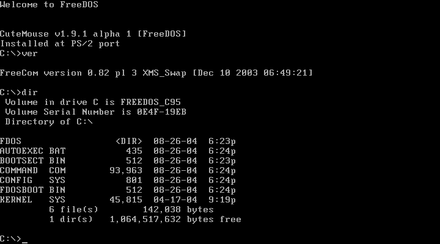
\includegraphics[width=0.7\linewidth]{Figuras/Ch01/fig36}
\end{frame}


\begin{frame}{Conceitos de hardware e software}
	\centering
	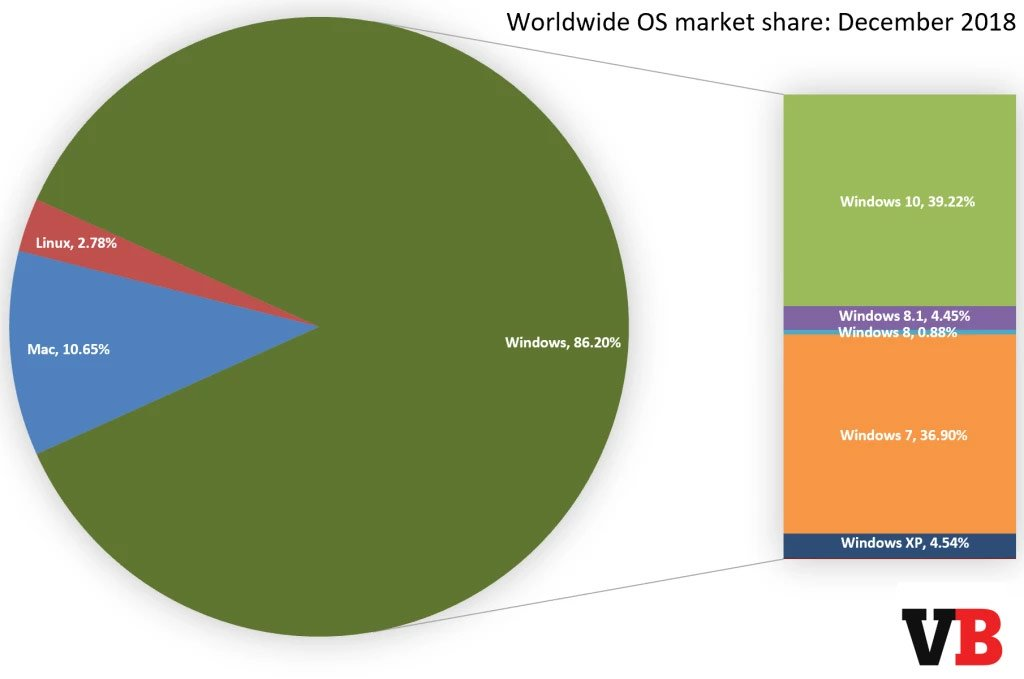
\includegraphics[height=0.9\textheight]{Figuras/Ch01/fig20}
\end{frame}


\begin{frame}{Conceitos de hardware e software}
	\begin{block}{Hardware (HW)}
		\begin{itemize}
			\item \textbf{Parte física} (tangível) do computador.
			\item Componentes eletrônicos, mecânicos, elétricos, cabos, etc.
			\item Pode ser desenvolvido para realizar diversas tarefas.
			\item As tarefas necessitam de entradas para fornecer saídas.
		\end{itemize}
	\end{block}

	\bigskip

	\centering
	\begin{tikzpicture}
		\node[rectangle, minimum height=1cm,minimum width=2cm,draw] (D) at (0,0) {Dados};
		\node[rectangle, minimum height=1cm,minimum width=2cm,draw,right=2cm of D] (P) {Processamento};
		\node[rectangle, minimum height=1cm,minimum width=2cm,draw,right=2cm of P] (I) {Informação};

		\draw[->,thick] (D.east) +(0.2cm,0) -- ($ (P.west)+(-0.2cm,0) $);
		\draw[->,thick] (P.east) +(0.2cm,0) -- ($ (I.west)+(-0.2cm,0) $);
		%		\draw[->] (D.east) -- (P.west);
	\end{tikzpicture}
\end{frame}


\begin{frame}{Conceitos de hardware e software}
	\begin{block}{Software (SW)}
		\begin{itemize}
			\item Parte lógica (intangível) do computador, responsável por ditar as \textbf{instruções} que o mesmo deve seguir a fim de \textbf{executar uma tarefa específica}.
			\item Um computador pode executar diversos tipos de
			      software:
			      \begin{itemize}
				      \item\normalsize sistemas operacionais;
				      \item\normalsize do pacote Office;
				      \item\normalsize navegadores;
				      \item\normalsize de uso específico.
			      \end{itemize}

		\end{itemize}
	\end{block}

	\centering
	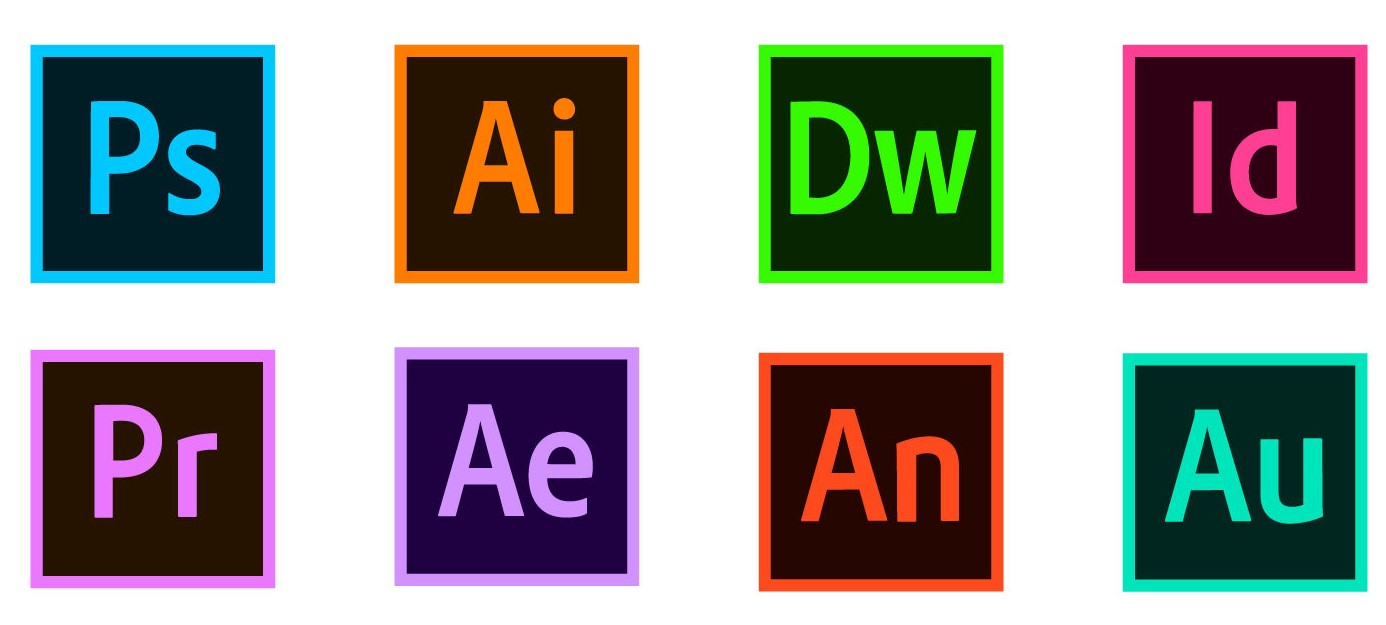
\includegraphics[width=0.6\linewidth]{Figuras/Ch01/fig22}
\end{frame}


\begin{frame}{Conceitos de hardware e software}
	\begin{block}{Software de sistema}
		\begin{itemize}
			\item Roda em segundo plano, gerenciando o \textit{hardware} e dando
			      suporte aos aplicativos, o sistema operacional.
		\end{itemize}
	\end{block}

	\begin{block}{Software de aplicativo}
		\begin{itemize}
			\item Responsável por auxiliar o usuário a realizar as suas tarefas.
			\item São bem mais específicos que um SO.
		\end{itemize}
	\end{block}

	%	\centering
	%	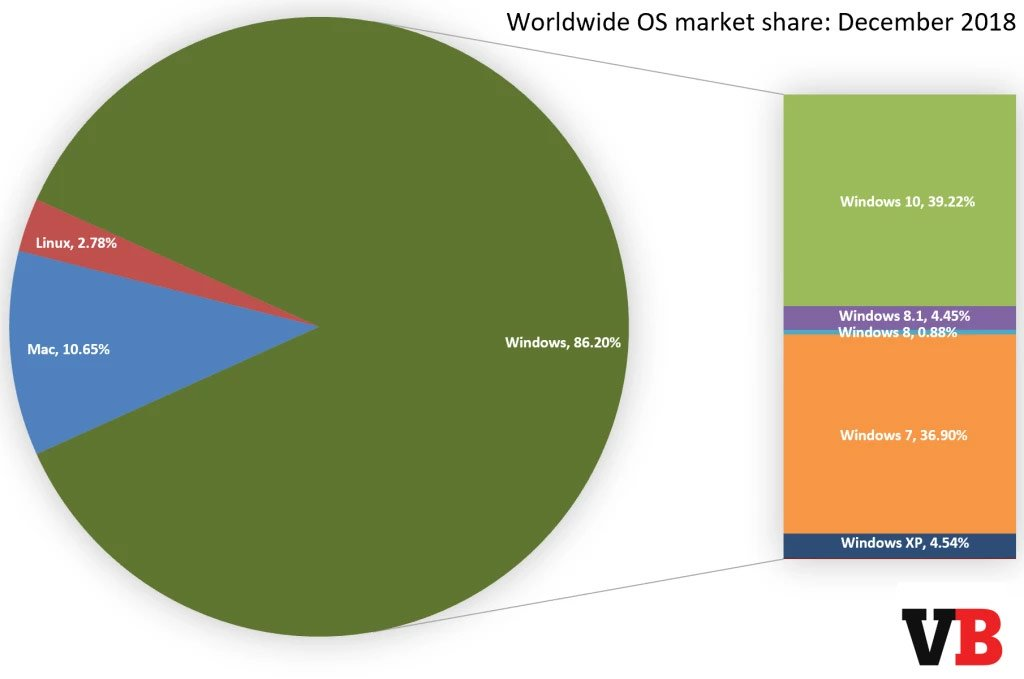
\includegraphics[width=0.4\linewidth]{Figuras/Ch01/fig20}
\end{frame}


\begin{frame}{Componentes de um computador}
	\begin{block}{}
		\textbf{Externamente}, nós vemos:
		\begin{itemize}
			\item gabinete (que é o computador em si);
			\item monitor;
			\item teclado;
			\item mouse;
			\item demais periféricos (estabilizador, impressora, scanner, etc.).
		\end{itemize}
	\end{block}

	\centering
	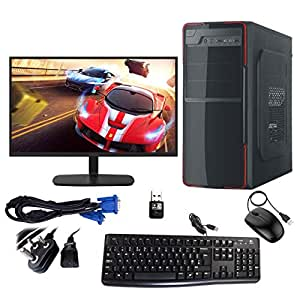
\includegraphics[width=0.35\linewidth]{Figuras/Ch01/fig23}
\end{frame}


\begin{frame}{Componentes de um computador}
	\begin{block}{Periféricos de entrada de dados}
		São todos aqueles que permitem ao usuário \textbf{enviar
			informações} para o sistema:
		\begin{itemize}
			\item teclado;
			\item mouse;
			\item scanner;
			\item microfone;
			\item tela touchscreen.
		\end{itemize}
	\end{block}

	\centering
	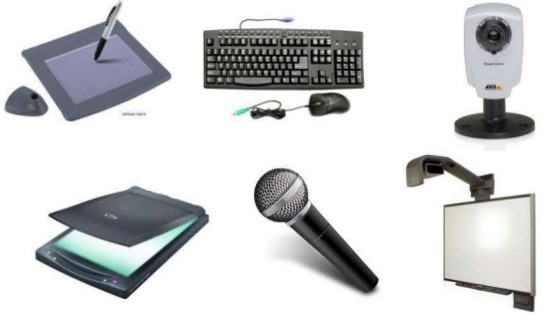
\includegraphics[width=0.45\linewidth]{Figuras/Ch01/fig27}
\end{frame}


\begin{frame}{Componentes de um computador}
	\begin{block}{Periféricos de saída de dados}
		São todos aqueles que \textbf{exibem dados visuais} ou sonoros
		para o usuário:
		\begin{itemize}
			\item monitor;
			\item auto-falantes;
			\item fones de ouvido;
			\item impressora.
		\end{itemize}
	\end{block}

	\centering
	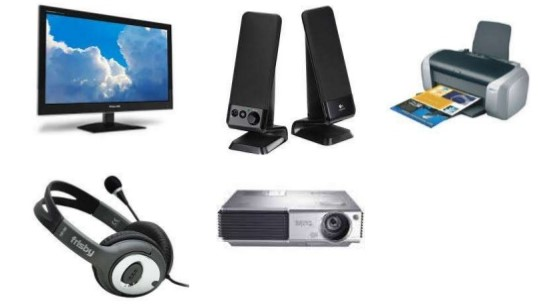
\includegraphics[width=0.6\linewidth]{Figuras/Ch01/fig26}
\end{frame}


\begin{frame}{Componentes de um computador}
	\begin{block}{Periféricos de entrada e saída de dados}
		São os que executam ambas funções.
		\begin{itemize}
			\item drive de CD, DVD (RW) e \textit{Blu-ray};
			\item pen drive.
		\end{itemize}
	\end{block}

	\begin{minipage}{0.49\linewidth}
		\centering
		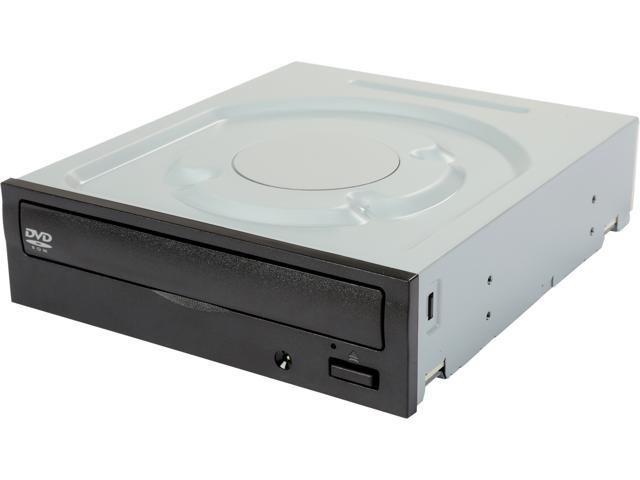
\includegraphics[width=1\linewidth]{Figuras/Ch01/fig27.1}
	\end{minipage}\hfill
	\begin{minipage}{0.49\linewidth}
		\centering
		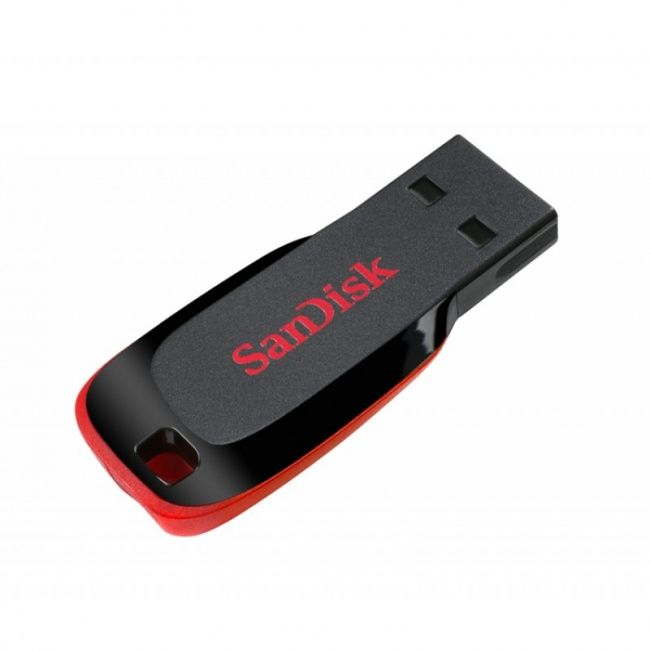
\includegraphics[width=1\linewidth]{Figuras/Ch01/fig27.2}
	\end{minipage}
\end{frame}


\begin{frame}{Componentes de um computador}
	\begin{block}{Periféricos de suporte}
		São todos aqueles que oferecem algum tipo de suporte às
		atividades do computador:
		\begin{itemize}
			\item filtros de linha, estabilizadores, nobreaks;
			\item roteadores;
			\item pendrives, HDs externos.
		\end{itemize}
	\end{block}

	\begin{minipage}{0.49\linewidth}
		\centering
		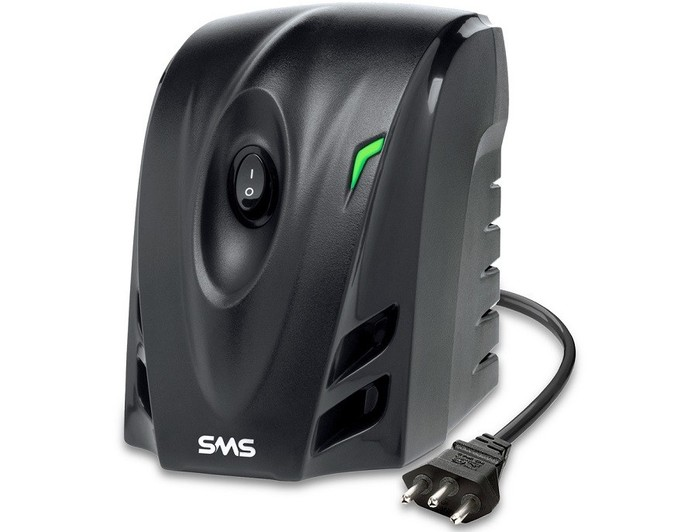
\includegraphics[width=0.8\linewidth]{Figuras/Ch01/fig28}
	\end{minipage}\hfill
	\begin{minipage}{0.49\linewidth}
		\centering
		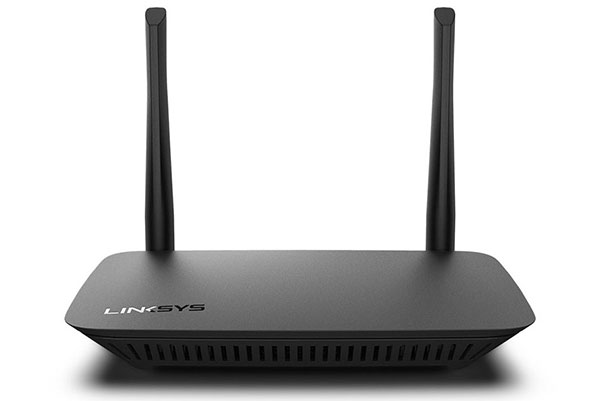
\includegraphics[width=1\linewidth]{Figuras/Ch01/fig29}
	\end{minipage}
\end{frame}


\begin{frame}{Componentes de um computador}
	\begin{block}{}
		O gabinete, por sua vez, também é composto por diversas
		partes:
		\begin{itemize}
			\item processador;
			\item memória principal (RAM) e secundária (HD/SSD);
			\item placa-mãe;
			\item fonte;
			\item leitores.
		\end{itemize}
	\end{block}

	\centering
	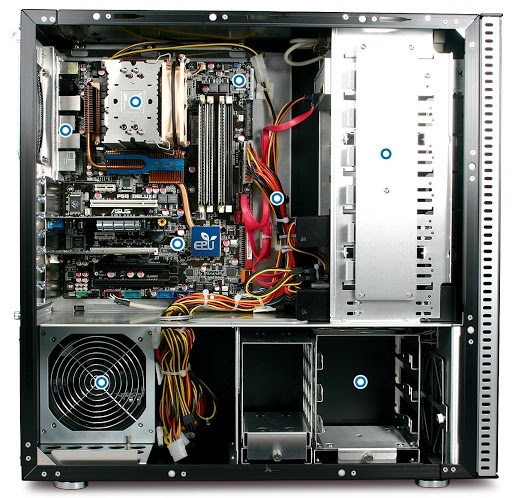
\includegraphics[width=0.35\linewidth]{Figuras/Ch01/fig24}
\end{frame}


\begin{frame}{Componentes de um computador}
	\begin{block}{Partes fundamentais de um computador}
		No gabinete, podemos encontrar as partes fundamentais,
		necessárias para o funcionamento do computador.
		\begin{itemize}
			\item processador;
			\item memórias;
			\item placa-mãe;
			\item fonte.
		\end{itemize}

		Outras partes importantes são:

		\begin{itemize}
			\item placa de vídeo;
			\item placa de áudio;
			\item placa de rede;
			\item leitores;
			\item conexões USB.
		\end{itemize}
	\end{block}

	%	\centering
	%	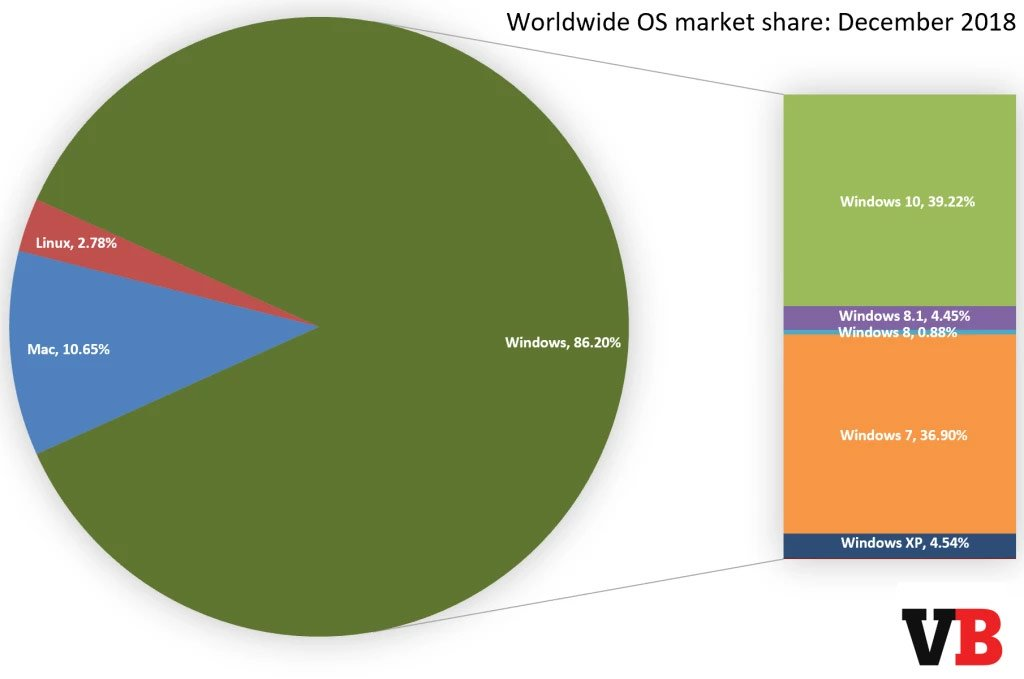
\includegraphics[width=0.4\linewidth]{Figuras/Ch01/fig20}
\end{frame}


\begin{frame}{Componentes de um computador}
	\begin{block}{Processador}
		\begin{itemize}
			\item Responsável por todo tipo de \textbf{processamento} no	computador.
			\item Recebe cada instrução do software e executa a operação definida.
		\end{itemize}

		Principais tipos de operações:
		\begin{itemize}
			\item cálculos lógicos-matemáticos;
			\item leitura ou armazenamento de dados em memória principal ou secundária.
		\end{itemize}
	\end{block}

	\centering
	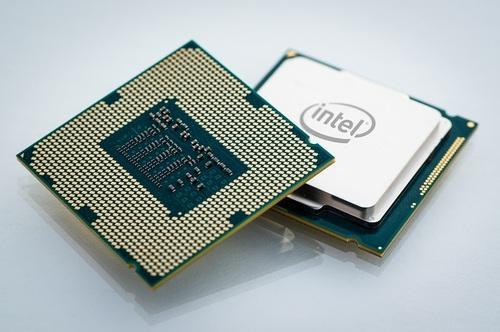
\includegraphics[width=0.45\linewidth]{Figuras/Ch01/fig31}
\end{frame}


\begin{frame}{Componentes de um computador}
	\begin{block}{Memórias}
		\begin{itemize}
			\item Responsáveis por armazenar as informações, seja de forma temporária (durante a execução de programas), ou de forma definitiva.
			\item Há dois tipos de memória:
			      \begin{itemize}
				      \item\normalsize principal;
				      \item\normalsize secundária.
			      \end{itemize}
		\end{itemize}
	\end{block}

	%	\centering
	%	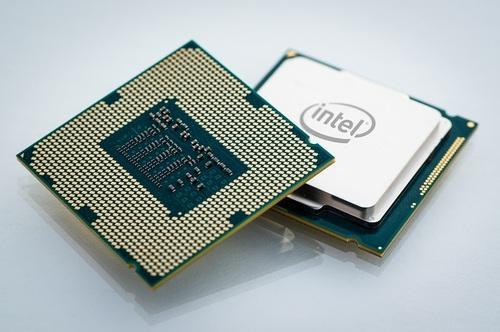
\includegraphics[width=0.4\linewidth]{Figuras/Ch01/fig31}
\end{frame}


\begin{frame}{Componentes de um computador}
	\begin{block}{Memória principal}
		\begin{itemize}
			\item Seu acesso é mais rápido, porém é \textbf{volátil}, isto é, as
			      informações permanecem na mesma somente enquanto o
			      computador estiver ligado.
			\item A \textbf{memória RAM} é uma memória principal.
		\end{itemize}
	\end{block}

	\centering
	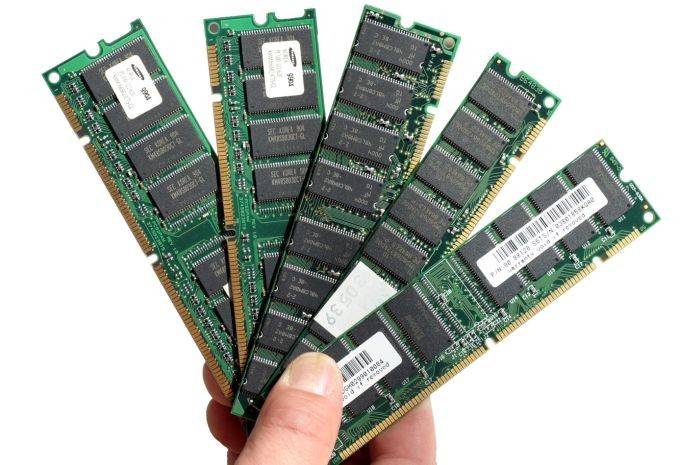
\includegraphics[width=0.6\linewidth]{Figuras/Ch01/fig35}
\end{frame}


\begin{frame}{Componentes de um computador}
	\begin{block}{Memória secundária}
		\begin{itemize}
			\item Seu acesso é mais lento, porém é a informação é armazenada de forma persistente, isto é, \textbf{não se perde após o desligamento do computador}.
			\item Discos rígidos (HD), discos de estado sólido (SSD), discos compactos (CD's) e pendrives são exemplos de memórias secundárias.
		\end{itemize}
	\end{block}

	\begin{minipage}{0.49\linewidth}
		\centering
		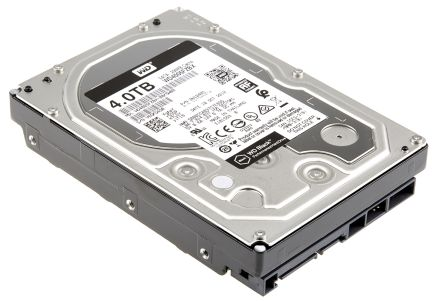
\includegraphics[width=1\linewidth]{Figuras/Ch01/fig34}
	\end{minipage}\hfill
	\begin{minipage}{0.49\linewidth}
		\centering
		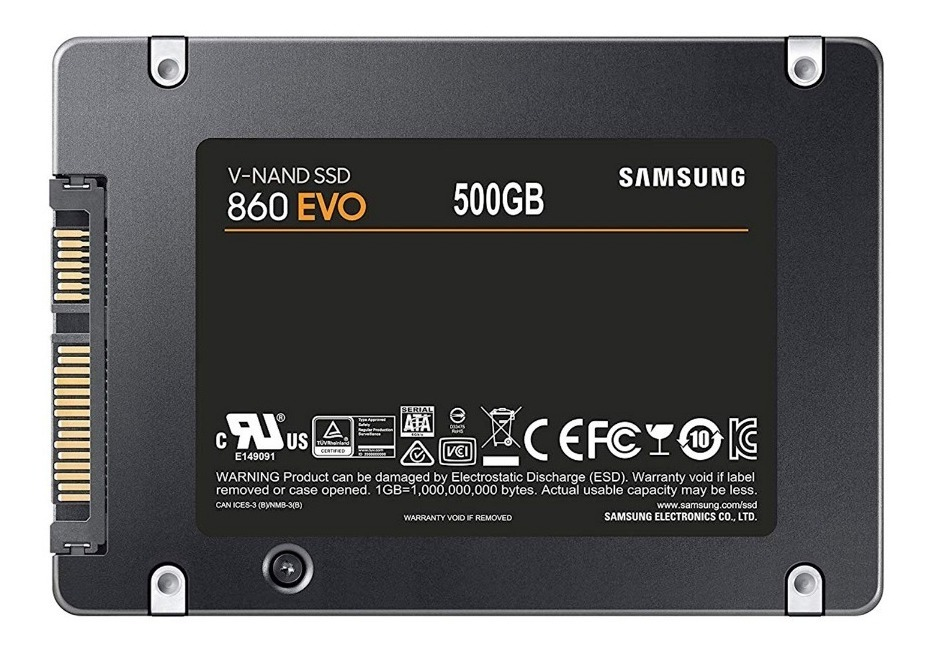
\includegraphics[width=1\linewidth]{Figuras/Ch01/fig33}
	\end{minipage}

\end{frame}


\begin{frame}{Componentes de um computador}
	\begin{block}{Placa-mãe}
		\begin{itemize}
			\item É a \textbf{principal peça do computador}, pois conecta todas as demais peças e periféricos.
			\item Podemos encontrar placas-mães com alguns dispositivos \textbf{integrados}.
			      \begin{itemize}
				      \item\normalsize Chamamos esses dispositivos integrados de \textit{on-board}.
				      \item\normalsize Por exemplo: todo notebook tem processador \textit{on-board}.
			      \end{itemize}
		\end{itemize}
	\end{block}

	\begin{minipage}{0.49\linewidth}
		\centering
		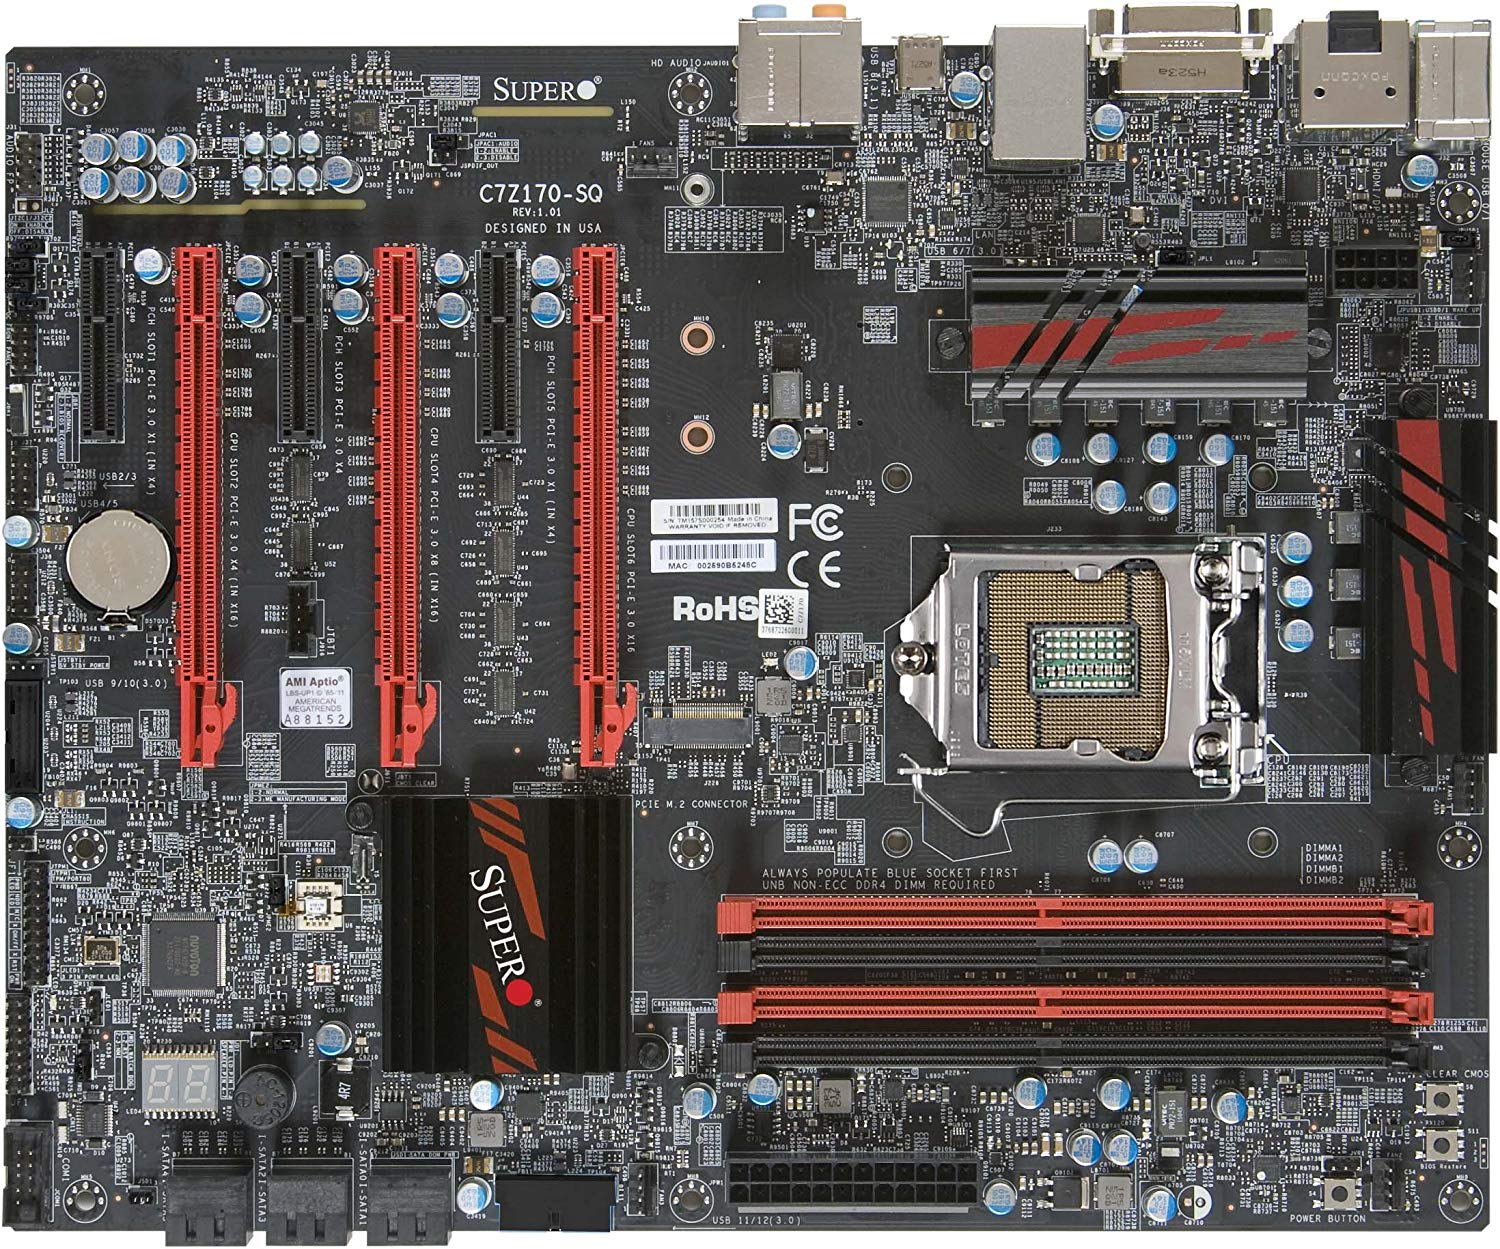
\includegraphics[width=0.8\linewidth]{Figuras/Ch01/fig32}
	\end{minipage}\hfill
	\begin{minipage}{0.49\linewidth}
		\centering
		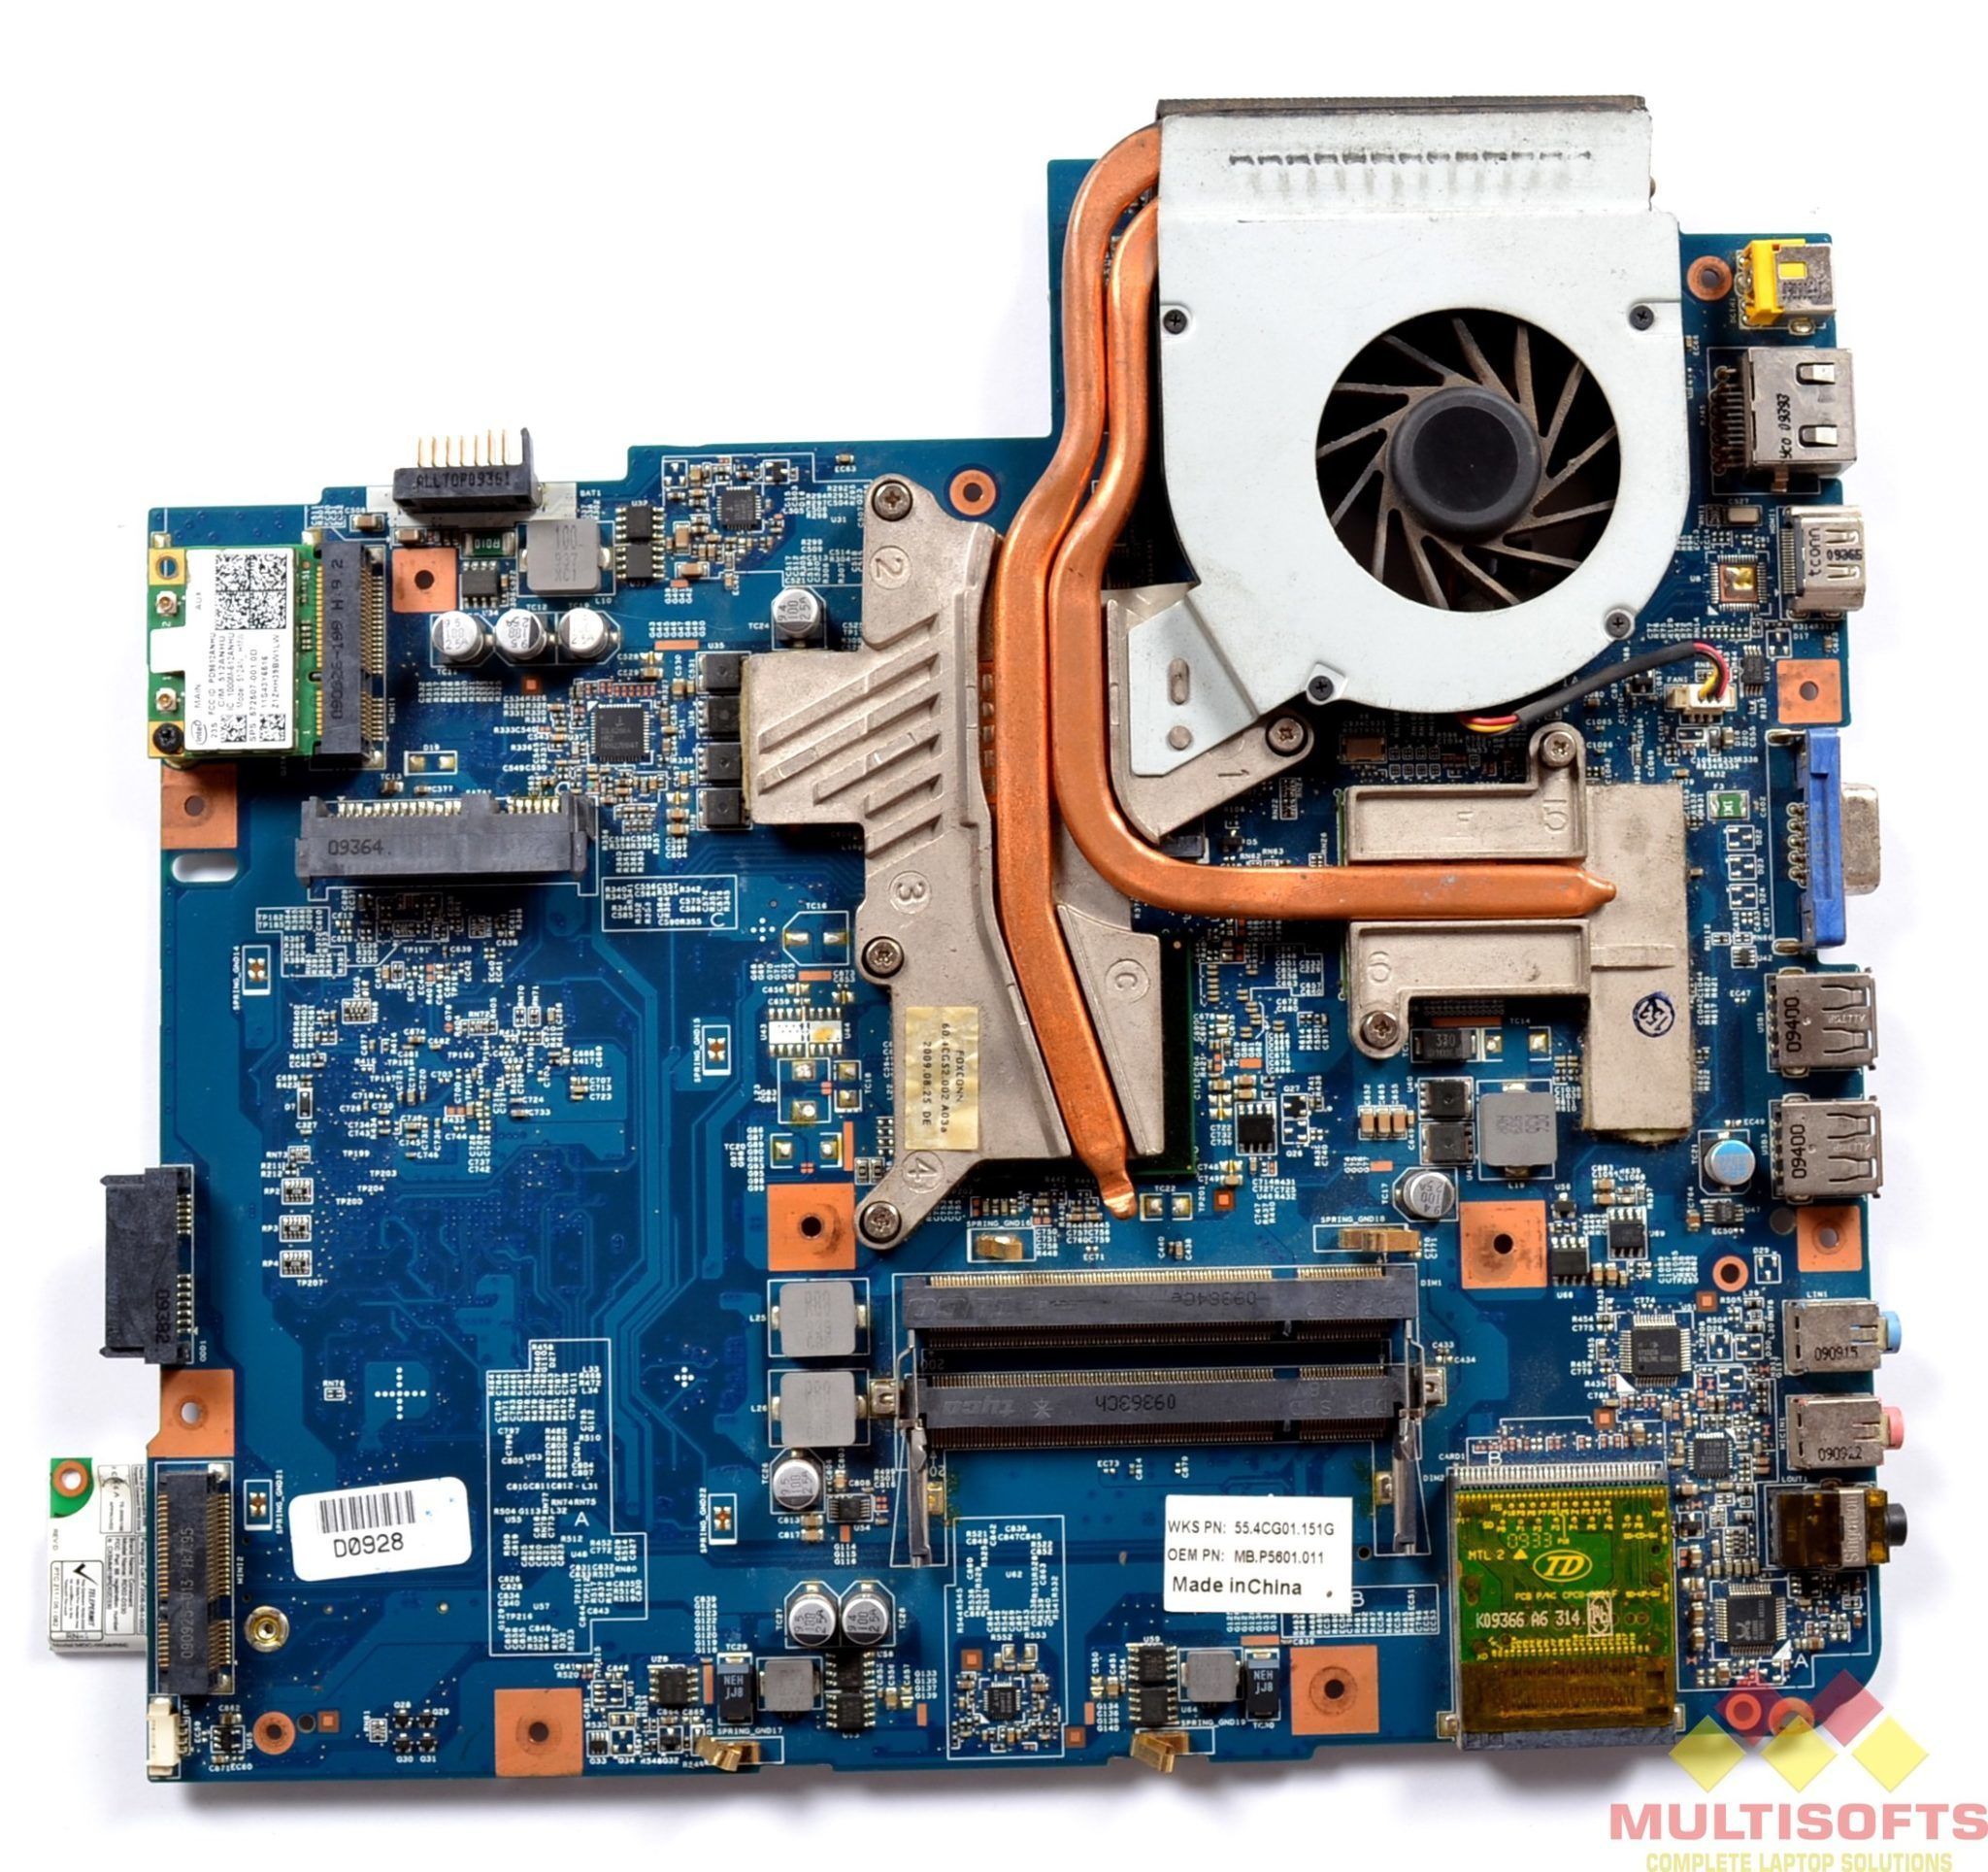
\includegraphics[width=0.8\linewidth]{Figuras/Ch01/fig30}
	\end{minipage}
\end{frame}


\section*{Exercícios}
\frame{
	\frametitle{Exercícios}
	\begin{block}{}
		01. Escreva com suas palavras o que é um computador e o que é informática.

		\medskip

		02. Quais são as vantagens de se utilizar um computador na vida profissional? E na vida pessoal?
	\end{block}
}

\section*{Referências}

\frame{
	\frametitle{Referências e Exercícios Complementares}
	\begin{itemize}
		\item Gammack, John G.; Hobbs, Valerie; Pigott, Diarmuid (2011). The Book of Informatics (em inglês) revisada ed. [S.l.]: Cengage Learning.
	\end{itemize}
	%\centering{\alert{Página 36 - \textbf{1.6.1 até 1.6.5, 1.6.17 até 1.6.19}}} \\
	%	\centering{\alert{Lista de exercícios 01}}
}